\documentclass[a4,center,fleqn]{NAR}

\usepackage{subcaption}
\usepackage{amsmath, amssymb, bm}
\usepackage{booktabs}
\usepackage{array}
\usepackage{multirow}
\usepackage{xcolor}
\usepackage{pifont}
\usepackage{microtype}

% ---- Custom commands ----
\newcommand{\cmark}{\ding{51}}
\newcommand{\xmark}{\ding{55}}
\newcommand{\hgt}{\textsc{HGT}}
\newcommand{\hgtrte}{\textsc{HGT+RTE}}
\newcommand{\gatv}{\textsc{GATv2}}
\newcommand{\eahgt}{\textsc{EA-HGT}}
\newcommand{\norm}[1]{\left\lVert#1\right\rVert}
\newcommand{\concat}{\,\|\,}

% Enter dates of publication
\copyrightyear{YYYY}
\pubdate{DD MM YYYY}
\pubyear{YYYY}
\jvolume{xx}
\jissue{xx}

%\articlesubtype{This is the article type (optional)}

\begin{document}

\title{THBKG: A Temporal Heterogeneous Biomedical Knowledge Graph for Quasi-Prospective Clinical Trial Advancement Prediction}

\author{%
Siu Pui Chung\,$^{1,3}$,
Claudia Cabrera\,$^{2,*}$,
Mani Mudaliar\,$^{3}$
and Arkaitz Zubiaga\,$^{1,*}$%


\address{%
$^{1}$School of Electronic Engineering and Computer Science, Queen Mary
University of London, United Kingdom,
$^{2}$Clinical Pharmacology, William Harvey Research Institute, Barts and
The London School of Medicine and Dentistry, Queen Mary University of
London, London, United Kingdom
and
$^{3}$Recursion Pharmaceuticals Inc, Salt Lake City, UT 84101, USA}

\history{%
Received YYYY-MM-DD;
Revised YYYY-MM-DD;
Accepted YYYY-MM-DD}

\maketitle

\begin{abstract}
Predicting which target--disease pairs will advance from Phase~II to
Phase~III clinical trials could improve how drug development resources
are allocated, but standard evaluation practices inflate performance by
allowing models to see evidence that post-dates the clinical decision.
Per-instance temporal masking removes this inflation, yet leaves 75.4\%
of Phase~II pairs with no direct target--disease evidence at their
decision point. We present the Temporal Heterogeneous Biomedical
Knowledge Graph (THBKG) and an end-to-end construction pipeline that
transforms Open Targets into a temporally-indexed heterogeneous graph,
enabling reconstruction of the evidence landscape at any historical
decision point. An Edge-Aware Heterogeneous Graph Transformer (EA-HGT)
trained on this graph outperforms a ridge regression baseline under
relative risk evaluation, with the advantage concentrated in
evidence-sparse strata where direct-edge models have no signal and
confirmed across 13 therapeutic areas. The THBKG and its construction
pipeline are provided as reusable resources for temporally faithful
clinical advancement prediction.
\end{abstract}


% ============================================================
\section{Introduction}
% ============================================================

Most drug candidates fail: approximately 90\% never reach regulatory
approval, and inadequate target--disease linkage accounts for 40--50\% of
Phase~II efficacy failures \citep{Sun2022WhyIt, Arrowsmith2013Trial2011-2012}. Because
target selection occurs early and propagates irreversibly into clinical
development, these failures are a principal driver of Eroom's Law, the
roughly nine-year doubling of inflation-adjusted cost per approved drug
observed since 1950 \citep{Scannell2012DiagnosingEfficiency}. Predicting which
target--disease pairs will advance through clinical trials, before
committing to expensive late-stage development, is therefore among the
most valuable capabilities a computational system could provide.

Czech et al.\ \citep{Czech2024CLINICALFORECASTING} showed that this is feasible. Using a
ridge regression model over 33 engineered biomedical evidence features,
they identify the top 2\% of target--disease pairs at 4--5$\times$ the
base advancement rate. Multimodal approaches that additionally incorporate
trial design and molecular properties can push accuracy higher still
\citep{Aliper2023PredictionIntelligence}, but Czech et al.'s result is notable because it
relies solely on biomedical evidence available before any specific trial
begins. The catch is that this performance holds only under a temporally
honest evaluation protocol, one that prevents the model from seeing
evidence that arrived after the clinical decision was made.

Biomedical evidence databases like Open Targets are cumulative snapshots
that reflect everything curated up to the present. Under standard
calendar-split evaluation, a single global cutoff year separates training
from test data, but test pairs that entered Phase~II years before the
cutoff still receive features computed from post-decision evidence. A
pair entering Phase~II in 2010 and evaluated with a 2015 cutoff absorbs
five years of post-decision publications, database updates, and
follow-on trial records into its feature representation. Successful
targets accumulate this post-decision evidence faster than unsuccessful
ones, because positive clinical results trigger accelerated publication,
curation, and further investigation. The result is that calendar-split
models partially learn to recognise that advancement \emph{already
happened}, rather than predicting that it \emph{will happen}.

Czech et al.\ address this with per-instance decision-aligned evaluation:
for each target--disease pair, all evidence is masked to the year of that
pair's Phase~II entry, so that the model sees only what was available when
the clinical decision was made \citep{Czech2024CLINICALFORECASTING}. This removes the
temporal inflation and produces honest performance estimates. But it also
exposes a structural problem: under proper temporal masking, 75.4\% of
Phase~II pairs have no direct target--disease evidence of any type at
their decision point. The curated evidence record simply has not caught up
to the clinical reality for most pairs. Among the minority with any direct
evidence, coverage is dominated by literature co-occurrence, a
volume-driven signal that reflects research attention more than
mechanistic validity. Direct-evidence models like the Czech et al.\ ridge
baseline cannot score pairs with empty feature vectors, so their
performance on the overall evaluation set is driven entirely by the
evidence-rich minority. Falaguera et al.\ \citep{Falaguera2025TemporalDiscovery} provide
supporting evidence that indirect paths can compensate for this sparsity:
44\% of novel drug targets carry indirect human genetic support compared
to 23\% with direct evidence alone, and 52\% have indirect non-clinical
support compared to 13\% directly, suggesting that multi-hop propagation
through a biomedical knowledge graph could extend predictive coverage to
pairs that direct-evidence models leave unscored.

We address this gap with the Temporal Heterogeneous Biomedical Knowledge
Graph (THBKG), constructed from Open Targets release 23.06. The graph
spans five entity types (targets, diseases, molecules, pathways, and Gene
Ontology terms) connected by 19 relation types (16 temporal, 3 static),
with temporally stamped edges indexed from 1995 to 2025. Each edge
timestamp records when the corresponding evidence first entered the
database. At inference time for any target--disease pair, all edges
post-dating that pair's Phase~II entry year are masked, reconstructing the
evidence landscape as it stood at the clinical decision point. Unlike
direct-evidence features, the graph's multi-hop structure (protein--protein
interactions, pathway memberships, functional annotations, drug modulation
links) survives temporal masking for most pairs, providing the encoder with
non-trivial input even when direct target--disease evidence is absent.

To validate that this structure carries advancement-predictive signal, we
train an Edge-Aware Heterogeneous Graph Transformer (\eahgt{}), extending
HGT \citep{Hu2020HeterogeneousTransformer} with continuous edge features (cumulative score and
Open Targets novelty score) as relation-type-specific multiplicative
modulations on the attention logit. The modification adds only two learned
parameters per relation type, keeping the encoder minimal so that
performance gains can be attributed to the graph structure and temporal
alignment rather than to model complexity.

This work makes three contributions:
\begin{enumerate}
\item The \textbf{THBKG}, a temporally-indexed heterogeneous biomedical
knowledge graph that supports per-instance reconstruction of the evidence
landscape at any historical clinical decision point, combining the
temporal masking called for by Czech et al.\ with the multi-hop
propagation structure motivated by Falaguera et al.

\item Results showing that \textbf{multi-hop graph propagation under
temporal constraints recovers advancement-predictive signal} for
evidence-sparse pairs that direct-edge models cannot score. Under
decision-aligned evaluation, \eahgt{} achieves RR@10 $\approx$ 6.02
versus 4.10 for the Czech et al.\ ridge regression baseline, and
RR@100 $\approx$ 4.82 versus 1.68, with the advantage concentrated in
the evidence-free and literature-only strata and confirmed across 13
therapeutic areas.

\item A framework for \textbf{quantifying temporal inflation risk}
through reconstruction of evidence subgraphs at shifted temporal offsets
around each pair's decision year, defining an empirical inflation
envelope for any evidence-based advancement prediction model.
\end{enumerate}


% ============================================================
\section{MATERIALS AND METHODS}
% ============================================================

\subsection{THBKG Construction}
\label{sec:thbkg_construction}

A knowledge graph provides a structured relational representation of
biomedical entities and their interactions. A \emph{heterogeneous}
knowledge graph admits multiple node and edge types, allowing a single
graph to simultaneously represent genetic associations, pathway
memberships, molecular interactions, and ontological hierarchies.

The THBKG is a \emph{discrete temporal heterogeneous graph} at yearly
resolution. Open Targets stores evidence as individual records: each one is
a single publication, variant annotation, animal model result, or other
observation linking a target to a disease through a specific datasource.
We aggregate these records into per-year cumulative snapshots: for each
(target, disease, datasource) triple, we compute the harmonic sum of all
evidence scores up to each year, producing a monotonically non-decreasing
trajectory of evidence strength over time. Each temporal edge in the
THBKG represents one year in this trajectory, carrying the cumulative
score and the Open Targets novelty score (Section~\ref{sec:ch4-scoring})
as continuous edge features. To avoid
storing unchanged values, we apply score-change event compression:
only years in which the cumulative score differs from the prior year
produce a stored edge, so every edge in the graph corresponds to a
genuine update in the evidence record. The result is a sequence of yearly
evidence landscape snapshots rather than a stream of individual events,
enabling reconstruction of the total evidence state at any historical
decision point through per-instance temporal masking: for a pair
$(v_t, v_d)$ with Phase~II entry year $y$, all edges with $t_{ij} \geq y$
are removed before any downstream computation.

\begin{figure}[t]
\centering
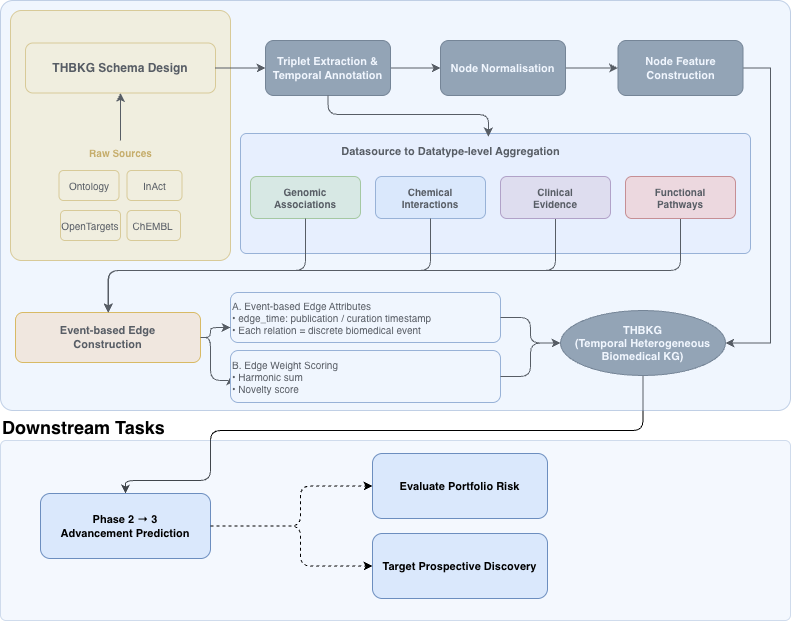
\includegraphics[width=\columnwidth]{figures/THBKG_pipeline_schema.drawio.png}
\caption{THBKG construction pipeline. Evidence records from Open Targets
release 23.06 are timestamped, scored via harmonic aggregation, and
assembled into a heterogeneous graph with per-instance temporal masking.}
\label{fig:thbkg_construction}
\end{figure}

\begin{figure}[t]
\centering
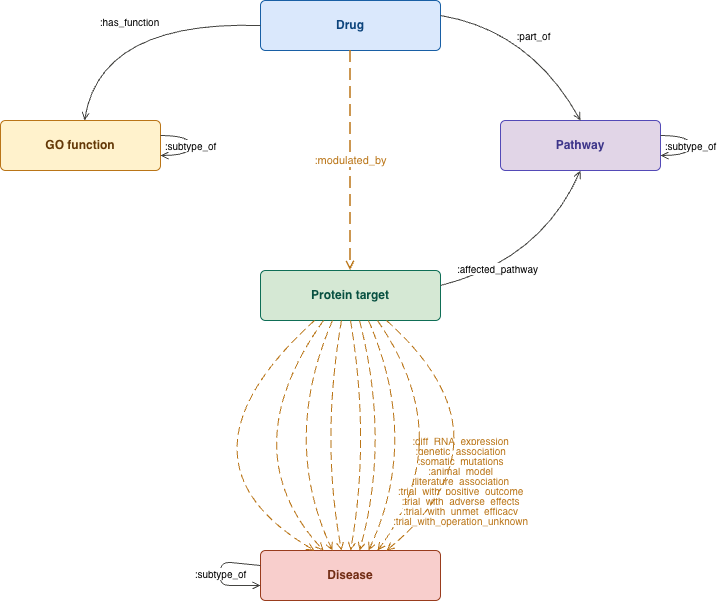
\includegraphics[width=\columnwidth]{figures/THBKG_schema.drawio.png}
\caption{THBKG schema. Five node types (target, disease, molecule,
Reactome pathway, GO term) are connected by 16 temporal edge types
(subject to per-instance masking) and 3 static structural edge types
(ontological hierarchies, always present regardless of cutoff year).
A separate \texttt{advancement} edge type serves as the prediction
target and is excluded from the GNN context graph.}
\label{fig:thbkg_schema}
\end{figure}


\subsubsection{Graph schema: entity and relation types.}

The THBKG is constructed from Open Targets release 23.06, a systematic
integration of multi-modal biomedical evidence linking targets and diseases
\citep{Ochoa2021OpenPrioritisation}. Five entity types are represented as node sets
(Table~\ref{tab:ch4-node-types}). Target--disease associations constitute
the primary prediction task; molecules, pathways, and Gene Ontology terms
provide the biological context through which those associations are
supported and through which multi-hop evidence paths are recovered
\citep{Narganes-Carlon2024GATher:Links}.

\begin{table}[h]
\tableparts{%
\caption{Node types in the THBKG with canonical identifiers, feature
dimensionality, and entity counts. Each node type carries a distinct
initial feature representation described in
Section~\ref{sec:thbkg_features}.}
\label{tab:ch4-node-types}%
}{%
\begin{tabular*}{\columnwidth}{@{}llrr@{}}
\toprule
\textbf{Node type} & \textbf{Identifier} & \textbf{Count} &
\textbf{Feat.\ dim} \\
\colrule
Target   & Ensembl gene ID & 19{,}316 & 56      \\
Disease  & EFO / MONDO ID  & 11{,}403 & 256     \\
GO term  & GO term ID      & 14{,}686 & 64      \\
Molecule & ChEMBL ID       &  2{,}703 & 1{,}024 \\
Reactome & Reactome ID     &  1{,}218 & 64      \\
\botrule
\end{tabular*}%
}{}
\end{table}

The graph comprises 19 edge relation types in total: 16 temporal and
3 static (Table~\ref{tab:edge_types_summary}; full details including
datasources in Supplementary Table~\ref{tab:edge_types_full}). All edges
carry a two-dimensional attribute vector
$\mathbf{f}_{ij} = [s_{ij},\; n_{ij}]^\top$, where $s_{ij}$ is the
cumulative association score at the edge's snapshot year and $n_{ij}$ is
the Open Targets novelty score at that year --- a logistic-decay function
of the recent jumps in the association's score trajectory, capturing how
recently the link acquired a burst of new evidence
(Section~\ref{sec:ch4-scoring}; \citealp{Falaguera2025TemporalDiscovery}).
For static edges, the attribute is fixed at $[0.0,\; 1.0]$.

\emph{Temporal edges} carry an \texttt{edge\_time} attribute recording the
year of the evidence snapshot (range 1995--2025) and are subject to temporal
masking during evaluation. \emph{Static structural edges} represent
ontological hierarchies (disease \texttt{is\_subtype\_of} (EFO/Disease
Ontology), GO term \texttt{is\_subtype\_of} (\texttt{is\_a} relationships),
and Reactome \texttt{is\_subpathway\_of}) which are definitional rather
than evidential and carry no temporal attributes; they form a persistent
scaffold always available regardless of the temporal cutoff.

Temporal edges span six categories of connectivity:

\begin{enumerate}
\item \textbf{Target--disease evidence edges} encode direct biomedical
associations from six Open Targets datasource categories: genetic
association (82{,}408 edges), animal model (442{,}082), literature
(237{,}795), RNA expression (171{,}555), somatic mutation (63{,}557),
and affected pathway (38{,}804).

\item \textbf{Clinical trial outcome edges} (disease $\rightarrow$ target)
are expanded into four outcome-specific relation types based on structured
ChEMBL metadata, mapping \texttt{clinicalStatus} and
\texttt{studyStopReasonCategories} fields to outcome categories following
\citet{Narganes-Carlon2024GATher:Links}: positive (56{,}190 edges), unknown/operational
(52{,}738), unmet efficacy (4{,}240), and adverse effects (2{,}115). During
training, clinical trial edges of all outcome types are excluded from the
GNN context graph to prevent label leakage.

\item \textbf{Pathway and functional annotation edges} connect targets to
Reactome pathways (\texttt{involved\_in}, 36{,}972 edges), diseases to
Reactome pathways (\texttt{associated\_with}, 3{,}639), and targets to Gene
Ontology terms (\texttt{has\_function\_in}, 256{,}090). These edges are
temporal, reflecting when the annotation first appeared in the respective
database.

\item \textbf{Drug modulation edges} (\texttt{modulated\_by},
target $\rightarrow$ molecule, 45{,}416 edges) connect targets to
compounds via ChEMBL compound--target activity records.

\item \textbf{Protein--protein interaction edges}
(\texttt{interacts\_with}, target $\rightarrow$ target, 659{,}444 edges)
are derived from IntAct and represent physical protein--protein
interactions. This is the largest single relation type in the graph and
provides the primary structural backbone for multi-hop propagation
between targets.

\item \textbf{Advancement edges} (\texttt{advancement},
target $\rightarrow$ disease, 34{,}410 edges) indicate that a
target--disease pair has advanced to a higher clinical phase at the given
year. These edges constitute the prediction target and are derived from
ChEMBL clinical trial records. Advancement edges are excluded from the
GNN context graph at both training and inference time.
\end{enumerate}

\begin{table}[h]
\tableparts{%
\caption{Edge types in the THBKG (19 total). \textbf{T}: temporal
(subject to per-instance masking); \textbf{S}: static (always present).
Clinical trial and advancement edges are excluded from the GNN context
graph. Full datasource details in Supplementary
Table~\ref{tab:edge_types_full}.}
\label{tab:edge_types_summary}%
}{%
\begin{tabular*}{\columnwidth}{@{}llrlc@{}}
\toprule
\textbf{Relation} & \textbf{Src $\rightarrow$ Dst} & \textbf{Count} &
\textbf{Type} \\
\colrule
\texttt{interacts\_with}       & target $\rightarrow$ target   & 659{,}444 & T \\
\texttt{animal\_model}         & target $\rightarrow$ disease  & 442{,}082 & T \\
\texttt{has\_function\_in}     & target $\rightarrow$ go       & 256{,}090 & T \\
\texttt{literature}            & target $\rightarrow$ disease  & 237{,}795 & T \\
\texttt{rna\_expression}       & target $\rightarrow$ disease  & 171{,}555 & T \\
\texttt{genetic\_association}  & target $\rightarrow$ disease  &  82{,}408 & T \\
\texttt{somatic\_mutation}     & target $\rightarrow$ disease  &  63{,}557 & T \\
\texttt{ct\_positive}          & disease $\rightarrow$ target  &  56{,}190 & T \\
\texttt{ct\_unknown}           & disease $\rightarrow$ target  &  52{,}738 & T \\
\texttt{modulated\_by}         & target $\rightarrow$ molecule &  45{,}416 & T \\
\texttt{affected\_pathway}     & target $\rightarrow$ disease  &  38{,}804 & T \\
\texttt{involved\_in}          & target $\rightarrow$ reactome &  36{,}972 & T \\
\texttt{advancement}           & target $\rightarrow$ disease  &  34{,}410 & T \\
\texttt{ct\_unmet\_efficacy}   & disease $\rightarrow$ target  &   4{,}240 & T \\
\texttt{associated\_with}      & disease $\rightarrow$ reactome &  3{,}639 & T \\
\texttt{ct\_adverse\_effects}  & disease $\rightarrow$ target  &   2{,}115 & T \\
\colrule
\texttt{is\_subtype\_of}       & go $\rightarrow$ go           &  14{,}415 & S \\
\texttt{is\_subtype\_of}       & disease $\rightarrow$ disease &  11{,}548 & S \\
\texttt{is\_subpathway\_of}    & reactome $\rightarrow$ reactome & 492    & S \\
\botrule
\end{tabular*}%
}{Sorted by count within temporal (T) and static (S) groups.}
\end{table}


\subsubsection{Temporal evidence aggregation.}
\label{sec:ch4-scoring}

Evidence accumulates monotonically over time. For each (target, disease,
datasource) triple and each year $Y \in \{1995, \ldots, 2025\}$, the
aggregated score incorporates all evidence records with publication or
annotation year $\leq Y$, producing a non-decreasing score trajectory that
reflects how biomedical confidence in an association builds as new
observations are recorded.

For non-clinical evidence, where multiple independent items provide
converging support, the aggregated score follows the Open Targets harmonic
sum convention \citep{Ochoa2021OpenPrioritisation}. Given $n$ evidence items with scores
sorted in descending order $s_1 \geq s_2 \geq \cdots \geq s_n$, the
aggregate is
\begin{equation}
    H = \frac{1}{\zeta(2)} \sum_{i=1}^{\min(n,\,50)} \frac{s_i}{i^2},
    \qquad \zeta(2) = \frac{\pi^2}{6} \approx 1.644,
    \label{eq:harmonic}
\end{equation}
where the $i^{-2}$ weighting ensures that the most informative items
dominate while additional corroborating evidence provides diminishing
marginal contributions, and $\zeta(2)$ normalises $H \in [0,1]$. For
clinical trial evidence, the score represents the highest phase reached by
a molecule against a target (an ordinal ceiling rather than an
accumulation of independent observations) and is therefore aggregated by
maximum rather than cumulative score.

Alongside the cumulative score $s_{ij}$, each edge carries the Open Targets
\emph{novelty} score \citep{Falaguera2025TemporalDiscovery}, a recency signal
derived from the score trajectory itself rather than from any clinical label.
Let $\Delta_p = \max(s_p - s_{p-1},\, 0)$ be the positive year-on-year jump in
the cumulative score at year $p$ (a ``peak'' in evidence accrual). The novelty
of the association at year $t$ is the maximum decayed contribution of any peak
within the preceding $W = 5$ years,
\begin{equation}
    n_{t} = \max_{\,t - W \leq p \leq t}\;
        \frac{\Delta_p}{1 + \exp\!\bigl(k\,((t - p) - m)\bigr)},
    \qquad k = 2,\; m = 3,
    \label{eq:novelty}
\end{equation}
following the parameterisation of \citet{Falaguera2025TemporalDiscovery}. Novelty is
high in the years immediately after an association gains new evidence and
decays back toward zero as that evidence ages, providing the encoder with a
signal of \emph{when} support arrived that is orthogonal to the cumulative
\emph{amount} of support encoded by $s_{ij}$. Novelty is computed per
datasource on the same yearly score series and aggregated to the datatype
level using the same two-level scheme as the scores.

Only (triple, year) combinations in which the aggregated score differs from
the preceding year are stored as events, so that each edge in the graph
corresponds to a genuine informational update in the evidence record. The
\texttt{edge\_time} attribute marks the year of this snapshot; the
\texttt{edge\_attr} records the two-dimensional feature vector
$[s_{ij}, n_{ij}]$ (cumulative score and novelty) at that year. This
score-change compression is a
lossless representation of the full monotonic trajectory: for any cutoff
year $y$, the correct score for a triple is the \texttt{edge\_attr} of the
most recent event with $t_{ij} < y$.

The resulting event list and static structural edges are assembled into a
single \texttt{HeteroData} object. For each temporal edge type, the graph
stores three tensors: \texttt{edge\_index} ($2 \times E$),
\texttt{edge\_time} (year of the evidence snapshot), and
\texttt{edge\_attr} ($E \times 2$, the cumulative score and novelty
score). Static edges are stored with \texttt{edge\_time}
set to a sentinel value (\texttt{INT64\_MIN}) and are never masked.


\subsubsection{Timestamp assignment.}

Edge timestamps are assigned following the timestamping methodology of
\citet{Falaguera2025TemporalDiscovery}, applied to Open Targets release 23.06. For each
evidence record, the primary source date is used in preference to the
curation date, reflecting the year in which the underlying observation was
originally reported rather than when it was deposited into a curated
repository (median curation lag: approximately 11 months
\citep{Falaguera2025TemporalDiscovery}). In the absence of a primary source date, the
curation date is used as a fallback. Overall, 99\% of temporal edges were
successfully timestamped. Static structural edges (disease ontology,
Gene Ontology hierarchy, Reactome pathway hierarchy) carry the sentinel
timestamp \texttt{INT64\_MIN}, indicating that they are always present
regardless of the temporal cutoff.

Per-source score thresholds are applied before edge construction to reduce
noise from high-volume, low-confidence datasources: EVA edges with score
$< 0.6$ and EuropePMC edges with score $< 0.3$ are excluded. The cumulative
score $s_{ij}$ and novelty score $n_{ij}$ are computed per retained
edge and stored as the two-dimensional edge attribute vector
$\mathbf{f}_{ij}$ described in Section~\ref{sec:formulation}.


\subsubsection{Node feature engineering.}
\label{sec:thbkg_features}

Each node type is initialised with a feature vector derived from its
biological or chemical properties, following \citet{Narganes-Carlon2024GATher:Links}.

\textbf{Targets} ($d = 56$) are represented by a multi-source vector combining gene
expression specificity and evolutionary constraint. Transcript abundance
across 81 cell types is quantified as normalised Transcripts Per Million
(nTPM) from single-cell RNA sequencing data, summarised by the
Jensen--Shannon Specificity score. Genetic constraint features include
Haploinsufficiency and Triploinsufficiency scores, the pLI/pLOEUF score
measuring tolerance to loss-of-function variants, and a Common Essential
flag identifying genes critical for cell survival.

\textbf{Diseases} ($d = 256$) are represented by sentence embeddings of disease names
and descriptions from the EFO ontology \citep{Ochoa2021OpenPrioritisation}, computed with a
pre-trained biomedical language model. This encodes semantic proximity
between disease entities in a continuous space, allowing the encoder to
generalise across related conditions even when direct graph connectivity
is sparse.

\textbf{GO terms and Reactome pathways} ($d = 64$ each) are represented by embeddings
learned from their respective ontology hierarchies (\texttt{is\_a} /
\texttt{part\_of} for GO; \texttt{is\_subpathway\_of} for Reactome) using
a graph auto-encoder, producing vectors that preserve structural proximity
within each ontology.

\textbf{Molecules} ($d = 1{,}024$) are represented by Morgan (circular)
fingerprints computed from canonical SMILES strings at radius 2 with a
bit-vector length of 1{,}024, encoding local chemical substructure relevant
to bioactivity.




% ============================================================
\subsection{Clinical Advancement Labels}
\label{sec:advancement_labels}

The binary advancement labels used to supervise link prediction were derived
following the per-instance, decision-aligned protocol introduced by Czech
et al.\ \citep{Czech2024CLINICALFORECASTING}, which we summarise here and extend with the
temporally masked graph described in
Section~\ref{sec:formulation}.

\subsubsection{Source data and trial identification.}

Clinical trial records were obtained from ClinicalTrials.gov, queried for
all interventional trials with at least one registered Phase~II arm and a
sponsor-reported primary completion date. Target--disease pairs were
extracted from each trial by mapping the registered intervention to a gene
target using the ChEMBL compound--target activity database
\citep{Gaulton2017The2017}, and mapping the registered condition to an EFO disease
ontology term via the Open Targets disease--ontology mapping. Only pairs
for which a unique target Ensembl gene identifier and a unique EFO disease
identifier could be assigned were retained. Trials involving combination
therapies with more than one active mechanism were excluded to avoid
confounding the target--disease evidence signal with multi-target
interactions.

\subsubsection{Advancement outcome definition.}

For each target--disease pair extracted from a Phase~II trial, the
advancement outcome was defined as a binary variable indicating whether the
pair subsequently entered a Phase~III trial within a fixed observation
window. A pair was labelled positive (advanced) if any Phase~III trial
registered after the Phase~II entry date listed the same target--disease
combination, as determined by exact match on the Ensembl gene and EFO
disease identifiers. A pair was labelled negative (did not advance) if no
such Phase~III registration was found within the observation window. Pairs
for which Phase~III status was ambiguous, including those with ongoing
Phase~II trials whose observation window had not closed, or those with
Phase~II trials terminated for non-efficacy reasons (e.g.\ safety signals
or commercial decisions), were excluded from the labelled set to avoid
label noise from administrative censoring.

\subsubsection{Decision-aligned evidence cutoff.}

The defining methodological contribution of Czech et al.\ is the
enforcement of a per-instance evidence cutoff: for each target--disease
pair, the evidence presented to the model is restricted to associations
whose timestamp predates the Phase~II entry date of that specific pair.
This per-instance cutoff eliminates the retrospective information leakage
that inflates performance in calendar-split designs, wherein a single
global training cutoff date permits test instances to be characterised by
evidence published after some pairs in the test set have already entered
the clinic. Under calendar-split evaluation, a model may effectively
observe the consequences of clinical decisions (accelerated publication of
results, rapid database curation of successful targets) when scoring pairs
at test time, producing optimistic performance estimates that do not
generalise to quasi-prospective or prospective deployment.

In the THBKG framework, we implement the per-instance cutoff directly
through the edge timestamp mechanism described in
Section~\ref{sec:formulation}: at inference time for a pair
$(v_t, v_d)$ with Phase~II entry year $y$, all graph edges with
$t_{ij} \geq y$ are masked before neighbourhood aggregation. The model
therefore receives exactly the evidence landscape that would have been
available to a human analyst making the prioritisation decision at year
$y$, with no access to subsequently curated associations.

\subsubsection{Dataset statistics and class balance.}

The labelled dataset follows the clinical advancement dataset of Czech
et al.\ \citep{Czech2024CLINICALFORECASTING}, spanning Phase~II trials registered between
1990 and 2025. Following their exclusion criteria, the final dataset
comprises positive and negative pairs at an approximate class ratio of
1:5, consistent with the empirical Phase~II to Phase~III advancement rate
reported by Wong et al.\ \citep{Wong2019EstimationParameters}. While the Czech et al.\
baseline models are trained with ridge regression on engineered features,
\eahgt{} is trained with the LambdaLoss formulation of LambdaRank
\citep{Wang2018TheOptimization} (the ungrouped, single-slate variant from the
allRank implementation \citep{Pobrotyn2020ContextAwareLearning}), which
directly optimises the ranking of target--disease pairs rather than
pointwise classification accuracy, aligning the training objective with
the RR@$N$ evaluation metric used in Czech et al.'s primary results.
Stratified sampling ensures that each training batch maintains
approximate class balance across therapeutic areas.

% ============================================================
\subsection{Problem Formulation}
\label{sec:formulation}
% ============================================================

Let $\mathcal{G} = (\mathcal{V}, \mathcal{E}, \mathcal{A}, \mathcal{R})$ denote
a temporal heterogeneous knowledge graph, where each node $v \in \mathcal{V}$
and each edge $e \in \mathcal{E}$ are associated with type mapping functions
$\tau(v) : \mathcal{V} \rightarrow \mathcal{A}$ and
$\phi(e) : \mathcal{E} \rightarrow \mathcal{R}$ respectively. For an edge
$e_{ij}$ connecting source node $v_i$ to target node $v_j$ via relation
$r \in \mathcal{R}$, the meta-relation is defined as the triple
$\langle \tau(v_i),\, \phi(e),\, \tau(v_j) \rangle$. Each edge additionally
carries a timestamp $t_{ij} \in \mathbb{R}$ recording when the underlying
evidence was first observed, and a continuous feature vector
\begin{equation}
    \mathbf{f}_{ij} = \bigl[s_{ij},\; n_{ij}\bigr]^\top \in \mathbb{R}^2,
\end{equation}
where $s_{ij}$ denotes the cumulative association score at the edge's
snapshot year and $n_{ij}$ denotes the Open Targets novelty score at that
year (Equation~\eqref{eq:novelty}).

The downstream task is link prediction over target--disease pairs: given the
graph state at a training cutoff $t^*$, predict whether a held-out
target--disease pair $(v_t, v_d)$ represents a valid therapeutic association.
For message passing, the graph is made undirected: for every relation type
$\langle \tau(v_i),\, r,\, \tau(v_j) \rangle$ we add a corresponding reverse
relation $\langle \tau(v_j),\, r^{-1},\, \tau(v_i) \rangle$ whose edges carry
the same timestamp $t_{ij}$ and edge-feature vector $\mathbf{f}_{ij}$ as their
forward counterparts, so that information can propagate along either
orientation of an evidence link. Reverse relations are kept type-distinct from
their forward relations, preserving the meta-relation structure on which the
heterogeneous encoders depend. We evaluate eight graph representation learning
configurations that differ in how they handle three independent properties of
the graph: (i) node and edge type heterogeneity, (ii) temporal edge
information, and (iii) continuous scalar edge features.


% ============================================================
\subsection{Baseline Models}
\label{sec:baselines}
% ============================================================

\subsubsection{Heterogeneous Graph Transformer (\hgt{}).}
\label{sec:hgt}

The Heterogeneous Graph Transformer~\citep{Hu2020HeterogeneousTransformer} parameterises attention
using node- and edge-type-specific weight matrices indexed by the meta-relation
triple. For each target node $v_t$ and source node $v_s$ connected via relation
$\phi(e)$, the heterogeneous mutual attention score is computed as
\begin{equation}
    \alpha_{ts} = \operatorname{softmax}_{s}\!\left(
        \frac{
            \left(\mathbf{Q}^{\tau(t)} \mathbf{h}_t\right)^\top
            \mathbf{W}^{\phi(e)}_{\mathrm{ATT}}\,
            \mathbf{K}^{\tau(s)} \mathbf{h}_s
        }{\sqrt{d}}
    \right),
    \label{eq:hgt-attn}
\end{equation}
where $\mathbf{Q}^{\tau(t)}, \mathbf{K}^{\tau(s)} \in \mathbb{R}^{d \times d}$
are node-type-specific query and key projections,
$\mathbf{W}^{\phi(e)}_{\mathrm{ATT}} \in \mathbb{R}^{d \times d}$ is an
edge-type-specific attention matrix, and $d$ is the hidden dimension per
attention head. The updated representation of $v_t$ is then
\begin{equation}
    \mathbf{h}'_t = \bigoplus_{\phi(e) \in \mathcal{R}}\;
        \sum_{s \in \mathcal{N}_{\phi(e)}(t)}
            \alpha_{ts}\cdot \mathbf{W}^{\phi(e)}_{\mathrm{MSG}}\,
            \mathbf{V}^{\tau(s)} \mathbf{h}_s,
    \label{eq:hgt-agg}
\end{equation}
where $\mathbf{W}^{\phi(e)}_{\mathrm{MSG}} \in \mathbb{R}^{d \times d}$ is an
edge-type-specific message projection, $\mathbf{V}^{\tau(s)}$ is a
node-type-specific value projection, and $\bigoplus$ denotes aggregation across
relation types (mean pooling in our experiments).

Although \hgt{} captures heterogeneity through its meta-relation-aware
parameterisation, the continuous edge features $\mathbf{f}_{ij}$ do not enter
any component of Equations~\eqref{eq:hgt-attn}--\eqref{eq:hgt-agg}. Two edges
of identical relation type receive identical attention scores and produce
identical messages regardless of differences in their cumulative score or
novelty score
values. We include standard \hgt{} as the primary heterogeneous baseline to
establish the performance ceiling of type-conditioned attention without
instance-level evidential weighting.

\subsubsection{Heterogeneous Graph Transformer with Relative Temporal Encoding (\hgtrte{}).}
\label{sec:hgt-rte}

The original HGT paper introduces a Relative Temporal Encoding (RTE) component
to handle dynamic heterogeneous graphs without constructing a separate snapshot
per time step~\citep{Hu2020HeterogeneousTransformer}. For each edge $e_{ij}$ observed at time
$t_{ij}$, the time gap relative to the current inference time $t$ is encoded as
\begin{equation}
    \mathrm{RTE}(\Delta t) = \mathbf{W}_{\mathrm{RTE}}\,
        \cos\!\left(\bm{\omega}\, \Delta t + \bm{\phi}_0\right),
    \qquad \Delta t = t - t_{ij},
    \label{eq:rte}
\end{equation}
where $\bm{\omega}, \bm{\phi}_0 \in \mathbb{R}^d$ are learnable frequency and
phase parameters and $\mathbf{W}_{\mathrm{RTE}} \in \mathbb{R}^{d \times d}$
is a learned projection. The temporal encoding is injected additively into the
value representation of each source node before message passing:
\begin{equation}
    \tilde{\mathbf{h}}_s = \mathbf{V}^{\tau(s)} \mathbf{h}_s +
        \mathrm{RTE}(\Delta t_{ts}),
    \label{eq:hgt-rte-value}
\end{equation}
with $\tilde{\mathbf{h}}_s$ replacing $\mathbf{V}^{\tau(s)} \mathbf{h}_s$ in
Equation~\eqref{eq:hgt-agg}. The attention computation in
Equation~\eqref{eq:hgt-attn} is unchanged. This formulation allows the model
to learn how much a source node's contribution should be discounted or amplified
based on the recency of the edge connecting it to the target, without requiring
discrete time-step snapshots.

We include \hgtrte{} as a direct ablation of \hgt{} to assess whether temporal
recency of evidence, as encoded by edge timestamps, provides signal beyond graph
structure and node features alone. The novelty score $n_{ij}$ in the edge
feature vector partially overlaps in meaning with RTE insofar as both relate to
evidence recency; comparing \hgtrte{} against models that use $n_{ij}$ directly
indicates whether a learned temporal encoding is redundant given an explicit
novelty feature, or whether it captures complementary temporal dynamics not
expressed by the scalar.

\subsubsection{Graph Attention Network v2 (\gatv{}).}
\label{sec:gatv2}

GATv2~\citep{Brody2021HowNetworks} addresses a known expressivity limitation in the
original GAT~\citep{Velickovic2017GraphNetworks}, where the ranking of neighbours is
independent of the query node (static attention). GATv2 reformulates attention
as a dynamic function of both source and target representations:
\begin{equation}
    \alpha_{ij} = \operatorname{softmax}_{j}\!\left(
        \mathbf{a}^\top \operatorname{LeakyReLU}\!\left(
            \mathbf{W}\,[\mathbf{h}_i \concat \mathbf{h}_j]
        \right)
    \right).
    \label{eq:gatv2-base}
\end{equation}
Because the score is computed over a concatenation of node features, continuous
edge features can be incorporated without architectural modification by
extending the concatenation:
\begin{equation}
    \alpha_{ij} = \operatorname{softmax}_{j}\!\left(
        \mathbf{a}^\top \operatorname{LeakyReLU}\!\left(
            \mathbf{W}\,[\mathbf{h}_i \concat \mathbf{h}_j \concat \mathbf{f}_{ij}]
        \right)
    \right),
    \label{eq:gatv2-edge}
\end{equation}
where $\mathbf{f}_{ij} \in \mathbb{R}^2$ is the edge feature vector. We apply
\gatv{} with edge features included via Equation~\eqref{eq:gatv2-edge}
throughout all \gatv{} conditions. Heterogeneity is handled through
\texttt{HeteroConv}, which instantiates a separate \gatv{} layer per edge type
and aggregates the resulting node representations, providing type-conditioned
message passing without the tightly integrated meta-relation parameterisation
of \hgt{}. We include \gatv{} as the primary edge-feature baseline, allowing
direct comparison with \hgt{}-family models at matched feature inputs.


% ============================================================
\subsection{Graph Encoder: Edge-Aware Heterogeneous Graph Transformer (\eahgt{})}
\label{sec:eahgt}
% ============================================================

The THBKG requires a graph encoder that can simultaneously exploit three
properties of its edges: heterogeneous relation types, continuous evidential
features ($s_{ij}$, $n_{ij}$), and temporal structure. The two baseline
families described above each address a subset of these requirements:
\hgt{} provides tightly integrated heterogeneous attention but is blind to
instance-level edge features; \gatv{} handles edge features naturally through
concatenation but integrates heterogeneity through an external aggregation
layer. We adopt \eahgt{}, an extension of \hgt{} that incorporates the
continuous edge feature vector $\mathbf{f}_{ij}$ directly into the attention
computation while preserving the full meta-relation-aware parameterisation of
the original architecture. The modification is deliberately lightweight ---
two learned parameters per relation type, so that observed performance gains
can be attributed to the THBKG's graph structure and temporal alignment rather
than to encoder complexity.

The key motivation is that $s_{ij}$ and $n_{ij}$ encode instance-level
evidential weight, properties that vary between edges of the same relation
type and are directly relevant to the downstream task of evidence sufficiency
scoring. In standard \hgt{}, $\alpha_{ts}$ is determined solely by node
representations and relation type; two edges that differ in cumulative score or
novelty receive the same attention weight. We address this by introducing a
relation-type-specific multiplicative modulation of the attention logit by
the edge features, extending HGT's existing multiplicative attention
structure to continuous per-edge attributes:
\begin{equation}
    \alpha_{ts} = \operatorname{softmax}_{s}\!\left(
        \frac{
            \left(\mathbf{Q}^{\tau(t)} \mathbf{h}_t\right)^\top
            \mathbf{W}^{\phi(e)}_{\mathrm{ATT}}\,
            \mathbf{K}^{\tau(s)} \mathbf{h}_s
        }{\sqrt{d}}
        \;\cdot\;
        \left(\mathbf{w}^{\phi(e)}_e\right)^\top \mathbf{f}_{ts}
    \right),
    \label{eq:eahgt-attn}
\end{equation}
where $\mathbf{w}^{\phi(e)}_e \in \mathbb{R}^2$ is a learned,
relation-type-specific projection vector mapping the two-dimensional edge
feature to a scalar that modulates the attention logit. The message and
aggregation steps are retained without modification from
Equation~\eqref{eq:hgt-agg}.

The multiplicative formulation is a natural extension of HGT's attention
mechanism, which already uses a relation-type-specific matrix
$\mathbf{W}^{\phi(e)}_{\mathrm{ATT}}$ to multiplicatively transform the
key--query interaction. The per-edge projection
$\mathbf{w}^{\phi(e)}_e$ adds instance-level modulation on top of this
type-level structure, allowing the model to learn that cumulative score and
novelty score contribute differently under different relation types.


% ============================================================
\subsection{Experimental Conditions}
\label{sec:conditions}
% ============================================================

To isolate the contribution of heterogeneous attention, temporal encoding, and
edge features independently, we evaluate the following conditions using a
shared evaluation protocol applied to the same graph and split:

\begin{table}[h]
\tableparts{%
\caption{Summary of experimental conditions. RTE: Relative Temporal Encoding.
$s_{ij}$: cumulative score. $n_{ij}$: Open Targets novelty score.}
\label{tab:conditions}%
}{%
\begin{tabular*}{\columnwidth}{@{}llll@{\extracolsep{\fill}}p{3.8cm}@{}}
\toprule
\textbf{ID} & \textbf{Model} & \textbf{RTE} & \textbf{Edge features} &
\textbf{Primary claim tested} \\
\colrule
B1 & \hgt{}    & \xmark & None               & Heterogeneous attention only \\
B2 & \hgtrte{} & \cmark & None               & Temporal recency without scalar features \\
B3 & \gatv{}   & \xmark & $s_{ij}$ only      & Score with partial heterogeneity \\
B4 & \gatv{}   & \xmark & $n_{ij}$ only      & Novelty with partial heterogeneity \\
B5 & \gatv{}   & \xmark & $s_{ij},\, n_{ij}$ & Both scalars with partial heterogeneity \\
\colrule
P1 & \eahgt{}  & \xmark & $s_{ij}$ only      & Score bias with full heterogeneity \\
P2 & \eahgt{}  & \xmark & $n_{ij}$ only      & Novelty bias with full heterogeneity \\
P3 & \eahgt{}  & \xmark & $s_{ij},\, n_{ij}$ & Both scalars with full heterogeneity \\
\botrule
\end{tabular*}%
}{B1--B5: baseline conditions. P1--P3: proposed \eahgt{} conditions.}
\end{table}

\noindent Conditions B3--B5 and P1--P3 share the same edge feature inputs but
differ in the attention mechanism, enabling a direct comparison of the two
architectural paradigms at matched feature configurations. The comparison
between B2 and P2 (or P3) additionally indicates whether RTE and the novelty
score $n_{ij}$ capture overlapping or complementary temporal signals: if B2
performs comparably to P2, learned temporal encoding may subsume the novelty
feature; if P3 substantially improves over B2, explicit scalar features carry
information beyond what a continuous time encoding captures.


\subsection{Link Prediction Head}
\label{sec:link_prediction_head}

After $L = 2$ layers of message passing, the encoder produces
$d$-dimensional embeddings $\mathbf{h}_t \in \mathbb{R}^{32}$ and
$\mathbf{h}_d \in \mathbb{R}^{32}$ for each target and disease node,
respectively. A three-layer MLP decoder maps their concatenation
$[\mathbf{h}_t \concat \mathbf{h}_d] \in \mathbb{R}^{64}$ to a scalar
ranking score:
\begin{align}
    \mathbf{z}_1 &= \operatorname{ReLU}(\mathbf{W}_1\,[\mathbf{h}_t \concat \mathbf{h}_d] + \mathbf{b}_1), &\quad &\mathbf{W}_1 \in \mathbb{R}^{32 \times 64}, \nonumber\\
    \mathbf{z}_2 &= \operatorname{ReLU}(\mathbf{W}_2\,\mathbf{z}_1 + \mathbf{b}_2), &\quad &\mathbf{W}_2 \in \mathbb{R}^{16 \times 32}, \nonumber\\
    \hat{y} &= \mathbf{w}_3^\top\,\mathbf{z}_2 + b_3, &\quad &\mathbf{w}_3 \in \mathbb{R}^{16}.
    \label{eq:decoder}
\end{align}
Dropout ($p = 0.1$) is applied after each ReLU activation. The output
$\hat{y}$ is an unbounded ranking logit used directly by the LambdaRank
loss; no sigmoid is applied, as the training objective optimises ranking
order rather than calibrated probabilities.

\textbf{LambdaRank loss.} \eahgt{} is trained with the LambdaLoss
formulation of LambdaRank \citep{Wang2018TheOptimization}, using the
ungrouped, single-slate variant from the allRank implementation
\citep{Pobrotyn2020ContextAwareLearning}: each training batch is treated as a
single ranked list, and pairwise logistic losses are weighted by the
absolute NDCG change from swapping each pair,
\begin{equation}
    \mathcal{L} = \sum_{\substack{(i,j):\\ y_i > y_j}}
        |\Delta\text{NDCG}_{ij}| \cdot
        \log\!\left(1 + e^{-\sigma(\hat{y}_i - \hat{y}_j)}\right),
    \label{eq:lambdarank}
\end{equation}
where $\sigma = 1.0$ controls the logistic slope and NDCG is truncated
at $k = 50$, matching the RR@$N$ cutoffs at which model selection and
reporting are performed. This directly aligns the training objective
with the RR@$N$ evaluation metric: both reward concentration of true
positives at the top of the ranked list. A therapeutic-area--grouped
variant (one ranked list per primary therapeutic area) was also
evaluated but rejected --- it gave no consistent improvement over the
ungrouped loss and exhibited high run-to-run variance in checkpoint
selection.


\subsection{Training and Evaluation Protocol}
\label{sec:training_evaluation}

\subsubsection{Dataset splits.}

The labelled dataset of Phase~II target--disease pairs and its
partitioning follow Czech et al.\ \citep{Czech2024CLINICALFORECASTING} exactly. Pairs are
split by the year of first Phase~II entry: the \textbf{training set}
consists of all pairs entering Phase~II between 1990 and 2015
(inclusive); the \textbf{evaluation set} consists of all pairs entering
Phase~II from 2016 onwards. Advancement ascertainment requires a
sufficient observation window after Phase~II entry; Czech et al.\ retain
pairs only where advancement status can be determined from subsequent
Phase~III registrations in the ClinicalTrials.gov record, consistent
with estimates that approximately half of Phase~II trials require more
than 2.9 years \citep{Wong2019}. This yields $N = 9{,}010$ pairs in the
evaluation set across all therapeutic areas, of which 9.01\% advanced
beyond Phase~II.

For both training and evaluation instances, temporal features are derived
using only evidence whose publication or annotation year precedes the
Phase~II entry year of that specific pair, i.e.\ the per-instance
decision-aligned cutoff of \citet{Czech2024CLINICALFORECASTING}. Genetic evidence features
are treated as static rather than temporal, following Czech et al.'s
empirical finding that genetic evidence exhibits low inflation risk and
that temporalising it does not improve predictive performance
(Section~2.7 of \citet{Czech2024CLINICALFORECASTING}).

\subsubsection{Therapeutic area stratification.}

Results are reported as equally-weighted averages across a subset of
therapeutic areas, following the selection criteria of Czech et al.\
\citep{Czech2024CLINICALFORECASTING}: a therapeutic area is retained if it contains at least
100 target--disease pairs with direct target--disease-specific evidence
of any kind within the evaluation set. The following therapeutic areas
are explicitly excluded regardless of size: \textit{biological\_process},
\textit{pregnancy or perinatal disease}, \textit{injury, poisoning or other
complication}, \textit{medical procedure}, and \textit{animal disease}, as
they are either not clinically relevant to drug target prioritisation or
are poorly represented. This yields 13 retained therapeutic areas, matching
the set used in Czech et al.'s primary performance figures.

\subsubsection{Metrics.}
\label{sec:metrics}

We adopt the evaluation metrics of Czech et al.\ \citep{Czech2024CLINICALFORECASTING} in full.

\textbf{Relative risk at $N$ (RR@$N$)} is the primary performance metric,
consistent with its use as the primary metric in Czech et al.\ and its
precedent in genetic support benchmarking studies
\citep{Nelson2015, King2019, Minikel2024}. For a ranked list of test
predictions sorted in descending order of predicted advancement probability,
RR@$N$ is defined as:
\begin{equation}
    \text{RR@}N =
    \frac{P(\text{advancement} \mid \text{rank} \leq N)}
         {P(\text{advancement} \mid \text{rank} > N)},
    \label{eq:rrn}
\end{equation}
that is, the probability of advancement among the top-$N$ predicted pairs
divided by the probability of advancement among all pairs ranked below $N$.
This formulation is identical to Equation~1 of \citet{Czech2024CLINICALFORECASTING}. An
RR@$N$ of 4.0 indicates that the top-$N$ pairs advance at four times the
rate of the remaining pairs.

We report RR@$N$ at $N \in \{10, 20, 30, 40, 50, 100\}$, matching the
cutoffs used in Czech et al.'s primary results table (Figure~4 of
\citet{Czech2024CLINICALFORECASTING}), as well as at the top-1\% and top-2\% cutoffs used
in their main performance figure. Results are reported as equally-weighted
averages across the 13 retained therapeutic areas, with 95\% Katz
log-method confidence intervals \citep{Katz1978ObtainingStudies} around each RR@$N$
point estimate.

\textbf{AUROC} and \textbf{Average Precision (AP)} are reported as
secondary metrics, again following Czech et al.\ \citep{Czech2024CLINICALFORECASTING}. Czech
et al.\ explicitly note that neither metric adequately captures behaviour
in the upper extremes of rankings (where performance is most relevant
for drug target prioritisation) due to the extreme sparsity of
direct target--disease evidence. These metrics are therefore reported for
completeness and comparability, but are not used as primary performance
indicators or for model selection. Model selection and hyperparameter
tuning are performed by validation set NDCG@50 under the decision-aligned
evaluation regime, matching the loss truncation $k = 50$.

\subsubsection{Hyperparameters.}

Table~\ref{tab:hyperparams} summarises the encoder and training
hyperparameters for the primary \eahgt{} configuration (P3). The hidden
dimension, number of attention heads, and number of layers were selected
by grid search over $d \in \{32, 64, 128\}$, heads $\in \{1, 2, 4\}$,
and layers $\in \{1, 2\}$; learning rate, weight decay, and the
LambdaRank slope $\sigma$ were optimised via Optuna on a log scale. All
hyperparameters were selected by NDCG@50 on the validation split under
the decision-aligned evaluation regime. During neighbourhood sampling,
each layer samples a fixed number of neighbours per edge type (20 at
layer 1, 10 at layer 2), selecting the most recent edges when the
neighbourhood exceeds the sample budget.

\begin{table}[h]
\tableparts{%
\caption{Hyperparameters for the \eahgt{} (P3) configuration.}
\label{tab:hyperparams}%
}{%
\begin{tabular*}{\columnwidth}{@{}l@{\extracolsep{\fill}}l@{}}
\toprule
\textbf{Parameter} & \textbf{Value} \\
\colrule
\multicolumn{2}{@{}l}{\textit{Encoder}} \\
Hidden / output dimension & 128 \\
Attention heads & 2 \\
Number of HGT layers & 2 \\
Dropout (encoder) & 0.2 \\
Edge feature dimension & 2 ($s_{ij}$, $n_{ij}$) \\
Neighbourhood sample (L1 / L2) & 20 / 10 \\
\colrule
\multicolumn{2}{@{}l}{\textit{Decoder}} \\
MLP layers & 256 $\rightarrow$ 128 $\rightarrow$ 64 $\rightarrow$ 1 \\
Dropout (decoder) & 0.1 \\
\colrule
\multicolumn{2}{@{}l}{\textit{Training}} \\
Loss & LambdaLoss / LambdaRank, ungrouped \\
 & ($k = 50$, $\sigma = 1.43$, lambdaRank scheme) \\
Graph orientation & undirected (reverse edges added) \\
Optimiser & AdamW \\
Learning rate & $4.35 \times 10^{-4}$ \\
Weight decay & $1.83 \times 10^{-3}$ \\
LR scheduler & CosineAnnealingLR ($\eta_{\min} = 10^{-6}$) \\
Epochs & 50 \\
Batch size & 512 \\
Gradient clipping & max\_norm $= 1.0$ \\
Early stopping & patience 5, metric NDCG@50 \\
\botrule
\end{tabular*}%
}{}
\end{table}

\noindent All experiments were run on the QMUL Apocrita HPC cluster
(Slurm) using a single NVIDIA A100 GPU.


% ============================================================
\section{RESULTS}
% ============================================================

\subsection{The Temporal Heterogeneous Biomedical Knowledge Graph}

The THBKG was constructed from Open Targets release 23.06, integrating
16 temporal edge types and 3 static ontological edge types across a
corpus of target--disease associations accumulated over two decades.
Figure~\ref{fig:thbkg_sunburst} presents the static edge composition of
the resulting graph as a sunburst diagram, with the inner ring partitioning
edges by datatype and the outer ring resolving individual datasources
nested within each category. After applying per-source score thresholds
(EVA $\geq$ 0.6, EuroPMC $\geq$ 0.3), the target--disease evidence edges
span six datatypes: \textit{genetic\_association},
\textit{somatic\_mutation}, \textit{affected\_pathway}, \textit{literature},
\textit{rna\_expression}, and \textit{animal\_model}, contributed by
sources including EVA, ChEMBL, and EuroPMC, among others. The distribution
is markedly heterogeneous: literature and genetic association edges account
for the plurality of the evidence graph, while clinical and pathway evidence
occupy substantially smaller fractions. Beyond direct target--disease
evidence, the THBKG includes protein--protein interaction edges (659{,}444
\texttt{interacts\_with} edges from IntAct), functional annotation edges
(256{,}090 \texttt{has\_function\_in} edges to GO terms), pathway membership
edges, and drug modulation edges, providing the structural backbone for
multi-hop propagation. This imbalance has direct implications for learned
representations, as embedding models trained on the full graph will
disproportionately encode signals from high-volume edge types irrespective
of their clinical relevance.

Figure~\ref{fig:thbkg_chord} examines the same graph through a temporal
lens, presenting chord diagrams at five cumulative cutoff years ($\leq$2005,
$\leq$2010, $\leq$2015, $\leq$2020, $\leq$2025). Each node in the chord
representation corresponds to a directed edge-type triple of the form
\textit{(source\_type $\rightarrow$ relation $\rightarrow$ target\_type)};
node arc size is proportional to edge count at the given cutoff, and ribbons
connect triples that co-occur on shared entities, weighted by their minimum
joint count. The progression across snapshots reveals a consistent and
structured pattern of graph densification. At the earliest cutoff
($\leq$2005), the graph is sparse and dominated by genetic association and
literature evidence; ribbon density is low, indicating that most entities are
supported by a single evidence type. By $\leq$2010, somatic mutation and known
drug edges begin to accumulate as cancer genomics resources and ChEMBL expand.
The late snapshots ($\leq$2020, $\leq$2025) are characterised by substantially
increased ribbon density, signalling that entities now accrue independent
corroboration across several datatypes simultaneously.

The temporal progression across cutoffs is consistent with the retrospective
analysis of Open Targets evidence timestamping reported by Falaguera et al.\
\citep{Falaguera2025TemporalDiscovery}, and reveals three analytically significant patterns.
First, evidence accumulation is datatype-specific and driven by curation
maturity rather than biological importance.
\texttt{animal\_model} edges (target $\rightarrow$ disease) dominate at
$\leq$2005 (64\% of total edges), reflecting the early systematic curation
of animal model phenotype data; Falaguera et al.\ identify the same
datatype as having an inflection point around 2005, earlier than all
other evidence categories, whose inflection occurs around 2015.
\texttt{rna\_expression} and \texttt{interacts\_with} (PPI) edges
accumulate substantially later, consistent with Falaguera et al.'s
observation of a surge in RNA expression recency peaks around 2015
following expanded integration of microarray data into the Expression Atlas. 
% The growth of \texttt{literature} edges, while steady across all
% cutoffs, does not correspond to proportional growth in unique novel
% targets, a pattern Falaguera et al.\ attribute explicitly to
% publication bias toward well-known genes and to the limitations of
% text-mining frameworks that cannot reliably distinguish a gene--disease
% mention from a validated association.
% This directly corroborates the streetlight framing adopted in this work: high
% literature edge volume encodes research attention rather than causal signal.
% Second, ribbon co-occurrence density increases markedly between $\leq$2010
% and $\leq$2020, indicating that models evaluated on the fully-observed graph
% will encounter richer multi-type neighbourhood structures than were available
% at any earlier decision point. The per-instance temporal masking described in
% Section~\ref{sec:conditions} is therefore essential to prevent structural
% leakage of this post-decision evidence.

\begin{figure}[t]
\centering
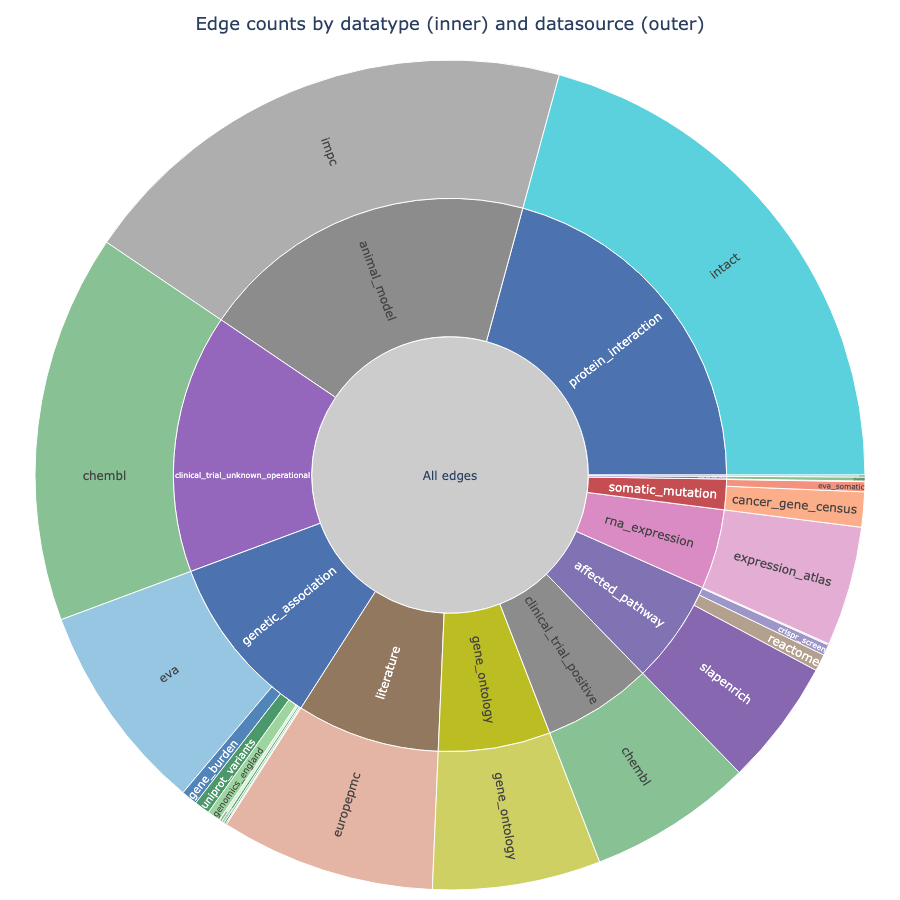
\includegraphics[width=\columnwidth]{figures/sunburst_diagram.drawio.png}
\caption{Sunburst diagram of the static edge distribution in the THBKG
(Open Targets release 23.06) across evidence datatypes and datasources.
The inner ring partitions edges by the seven high-level Open Targets
evidence categories; the outer ring resolves individual datasources
(e.g.\ EVA, ChEMBL, EuroPMC). Arc area is proportional to edge count
after applying per-source score thresholds (EVA $\geq$ 0.6,
EuroPMC $\geq$ 0.3).}
\label{fig:thbkg_sunburst}
\end{figure}

\begin{figure*}[t]
\centering
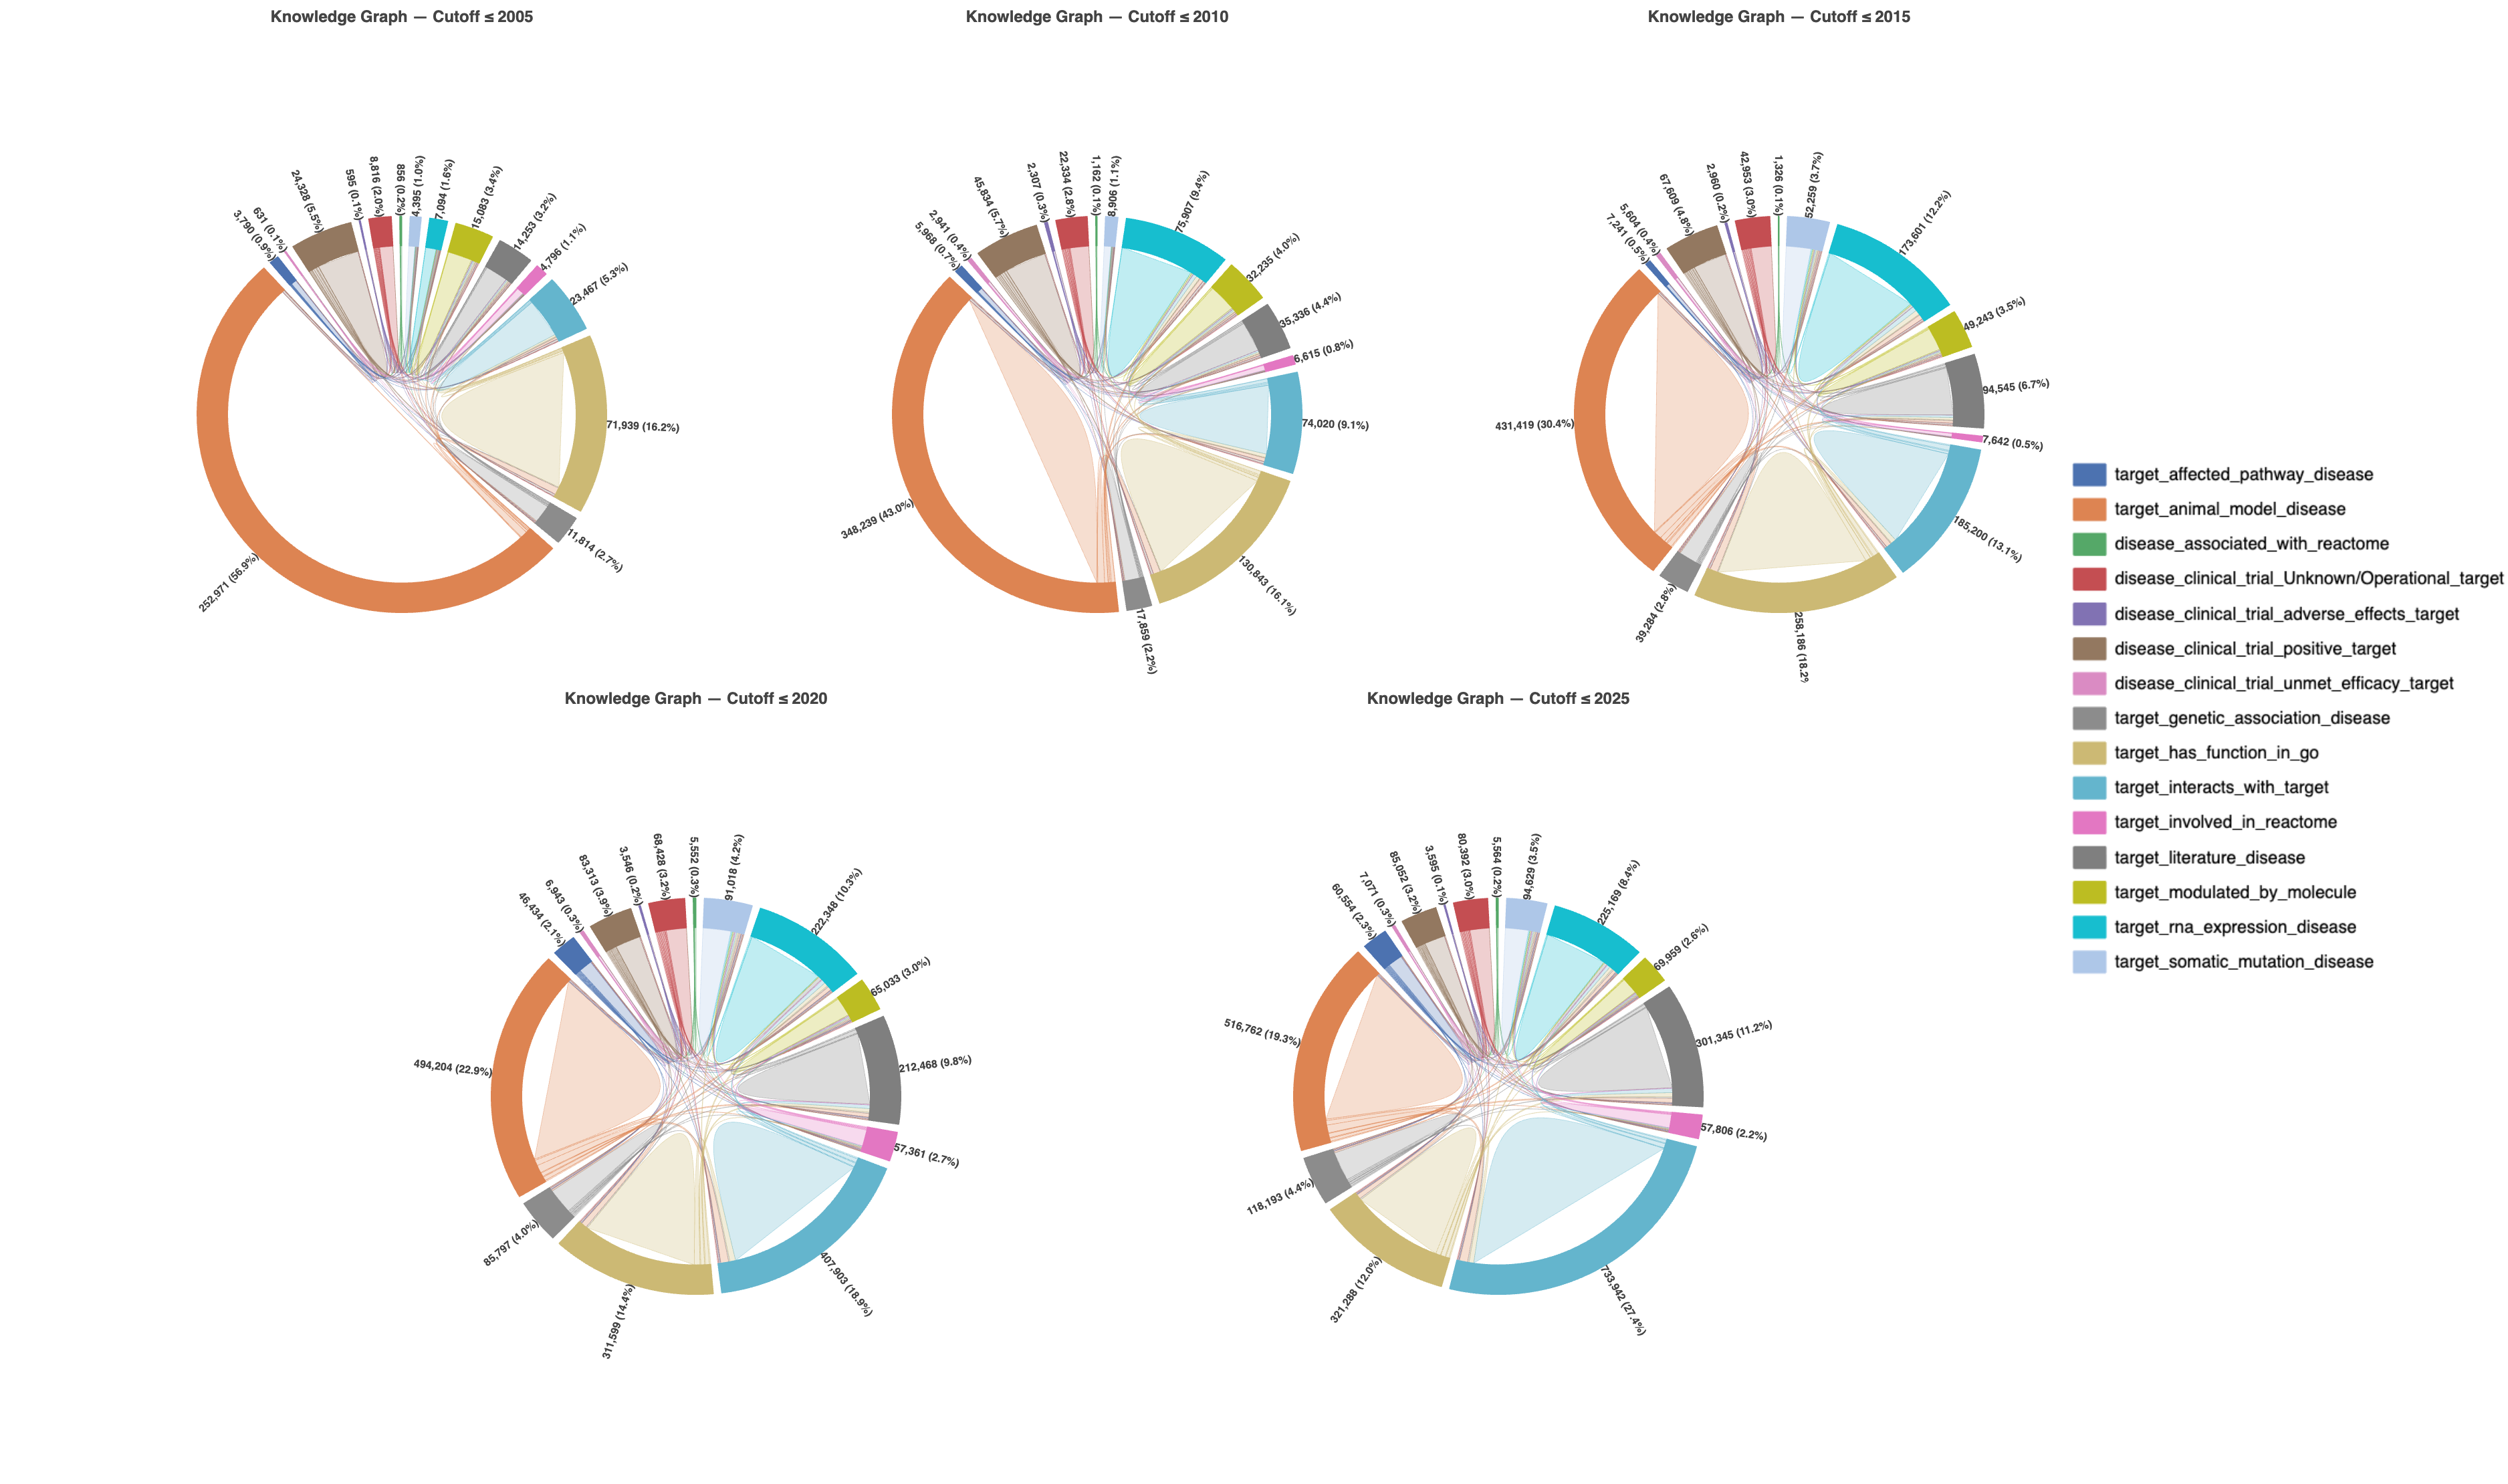
\includegraphics[width=\textwidth]{figures/chord_diagram.drawio.png}
\caption{Chord diagrams of the THBKG at five cumulative temporal cutoffs
($\leq$2005, $\leq$2010, $\leq$2015, $\leq$2020, $\leq$2025). Each
node represents a directed edge-type triple; arc size is proportional to
edge count at that cutoff. Ribbons connect triples that co-occur on
shared entities, weighted by their minimum joint count. Colour encoding
is consistent across all panels and with Figure~\ref{fig:thbkg_sunburst}.}
\label{fig:thbkg_chord}
\end{figure*}



\subsection{Multi-Hop Propagation on the THBKG Outperforms Direct-Edge Ridge Regression Baseline}
\label{sec:main_results}

% NOTE: All results are based on Open Targets release 23.06. The full
% pipeline is anchored at this release; re-running against 25.06 may
% shift absolute RR values as evidence coverage evolves. Ablation
% analysis across conditions B1--P3 is in preparation.

We compare the proposed \eahgt{} model (condition P3, trained with
the ungrouped LambdaLoss objective) against the ridge regression
baseline of Czech et al.\ \citep{Czech2024CLINICALFORECASTING} (RDG) and the Open
Targets global association score (OTS) on the held-out evaluation set
of $N = 9{,}010$ Phase~II target--disease pairs.

\subsubsection{Global classification metrics.}

On threshold-free classification metrics averaged across 13 therapeutic
areas, \eahgt{} attains a higher average precision than either
reference: AUROC $\approx$ 0.59 and average precision $\approx$ 0.19,
compared to $\approx$ 0.64 and 0.12 for RDG. OTS falls below both
(AUROC $\approx$ 0.49, AP $\approx$ 0.09), reflecting the absence of
temporal calibration. \eahgt{} trails RDG slightly on AUROC
but exceeds it on average precision, the metric more sensitive to
performance in the positive-enriched head of the ranking, where
prioritisation value is concentrated.

\subsubsection{Relative risk at top-$N$.}

At the top of the ranking, \eahgt{} substantially outperforms RDG at
every cutoff (Table~\ref{tab:rr_main}, Figure~\ref{fig:rr_by_limit}).
At $N = 10$, \eahgt{} achieves RR $\approx$ 6.02 compared to 4.10 for
RDG (+1.92). The advantage holds across all cutoffs from $N = 10$ to
$N = 100$, with the largest absolute gains in the $N = 30$--$50$ range
($\Delta$RR up to +4.25 at $N = 50$). At $N = 100$, \eahgt{} maintains
RR $\approx$ 4.82 versus 1.68 for RDG --- a $2.9\times$ enrichment ---
showing that the advantage persists across the actionable range of the
ranking. The 95\% Katz confidence interval for \eahgt{} lies entirely
above the RDG point estimates across all cutoffs
(Figure~\ref{fig:rr_by_limit}).

\begin{table}[h]
\tableparts{%
\caption{Relative risk at top-$N$ (RR@$N$) for \eahgt{} (P3) and RDG,
computed as the mean across 13 primary therapeutic areas (Open Targets
23.06). $\Delta$ denotes the difference P3 $-$ RDG. 95\% Katz confidence
intervals for \eahgt{} are shown in Figure~\ref{fig:rr_by_limit}.}
\label{tab:rr_main}%
}{%
\begin{tabular*}{\columnwidth}{@{}r@{\extracolsep{\fill}}rrr@{}}
\toprule
$N$ & RDG & \textbf{\eahgt{}} & $\Delta$ \\
\colrule
10  & 4.10 & \textbf{6.02} & +1.92 \\
20  & 2.74 & \textbf{5.70} & +2.96 \\
30  & 2.45 & \textbf{5.84} & +3.39 \\
40  & 2.27 & \textbf{5.88} & +3.61 \\
50  & 1.94 & \textbf{6.19} & +4.25 \\
60  & 1.78 & \textbf{5.93} & +4.15 \\
70  & 1.74 & \textbf{5.45} & +3.71 \\
80  & 1.73 & \textbf{5.09} & +3.37 \\
90  & 1.66 & \textbf{4.94} & +3.28 \\
100 & 1.68 & \textbf{4.82} & +3.14 \\
\botrule
\end{tabular*}%
}{}
\end{table}

\begin{figure}[t]
\centering
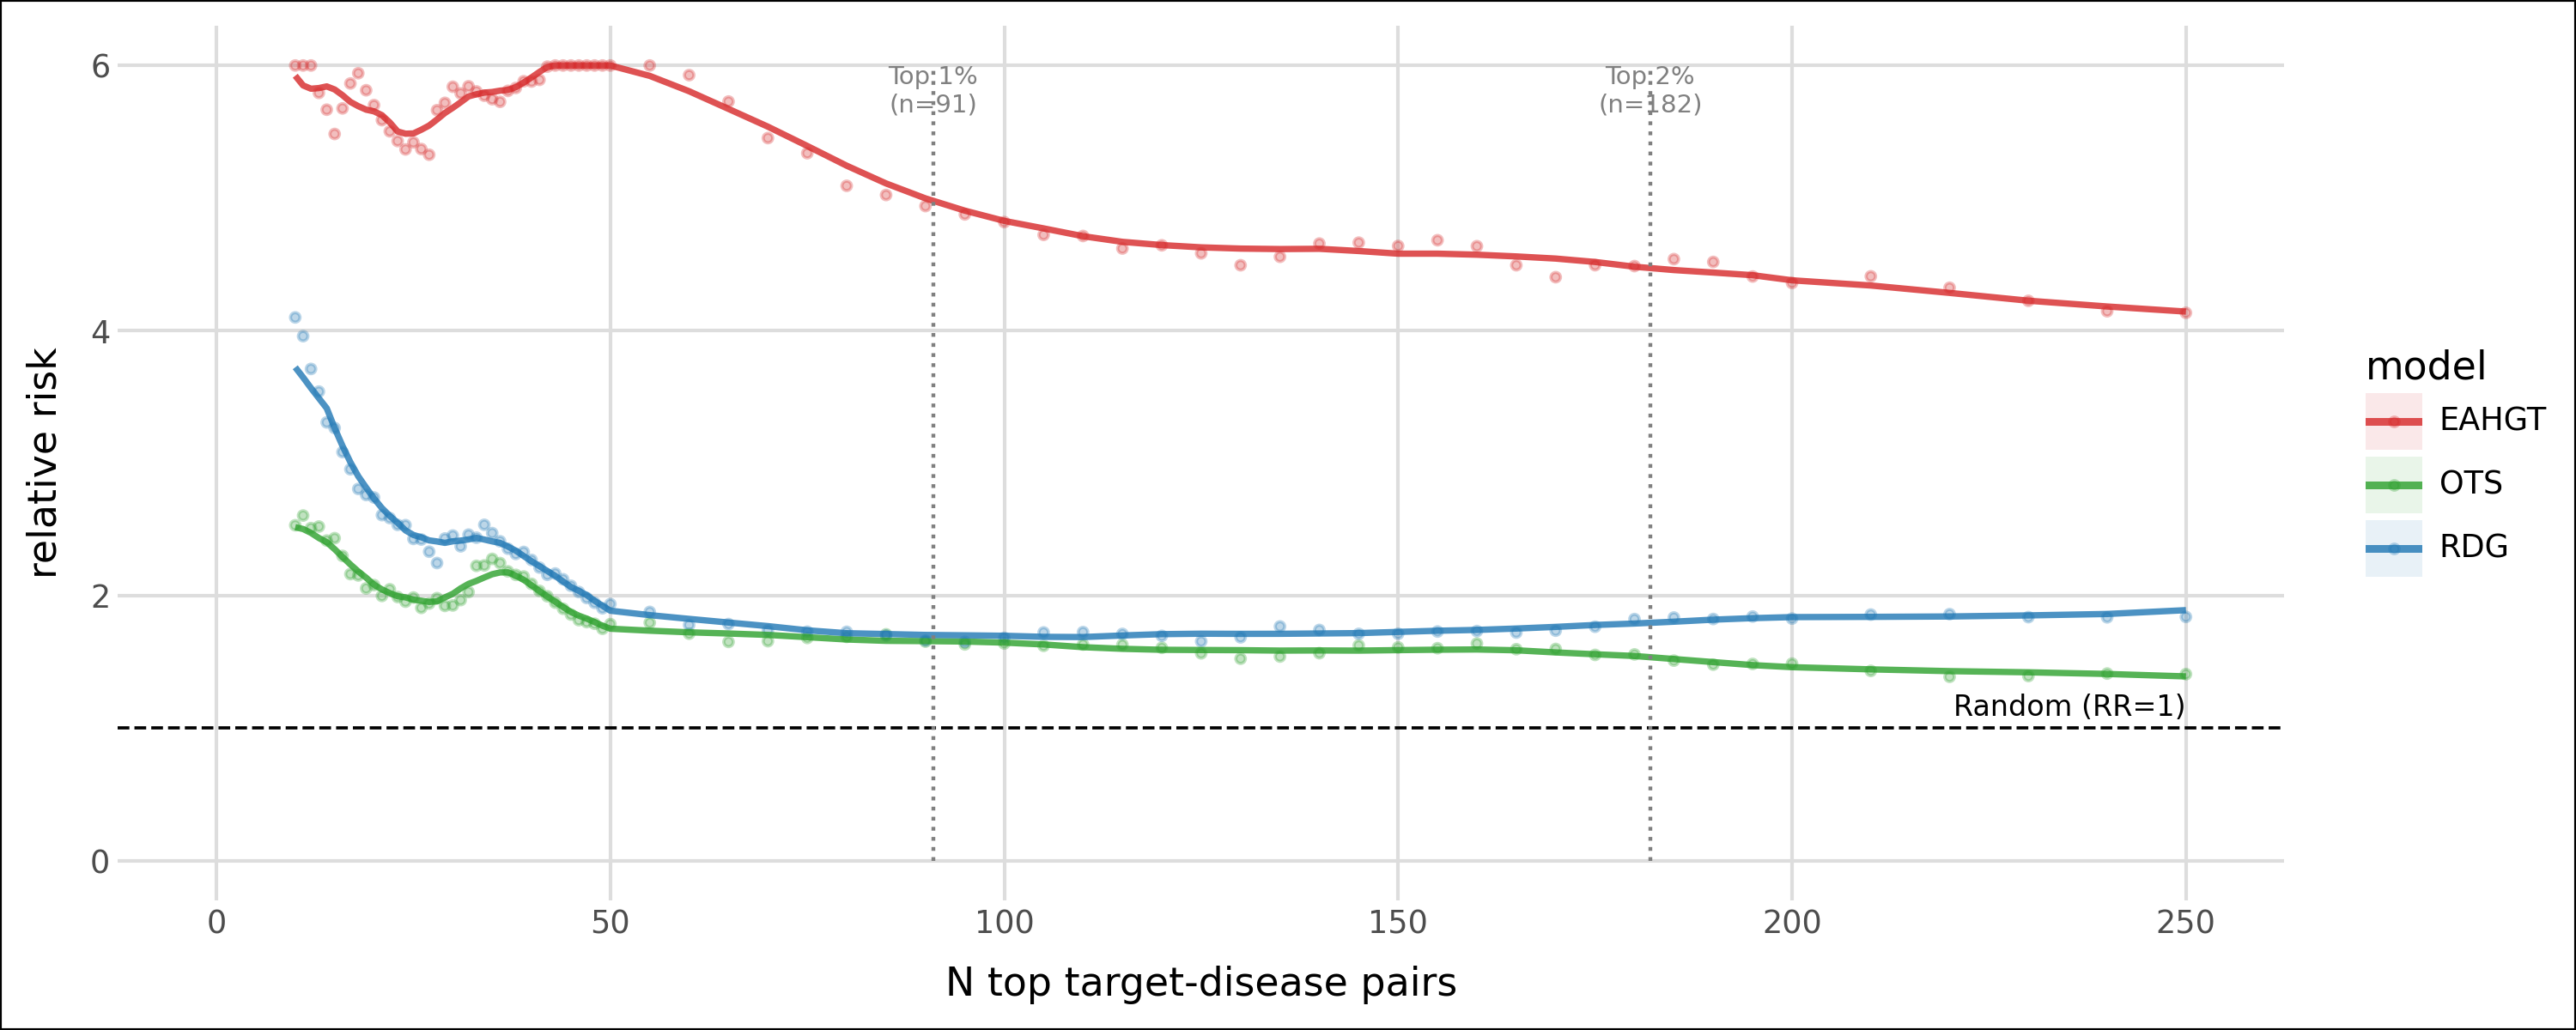
\includegraphics[width=\columnwidth]{figures/results/relative_risk_by_limit_katz95.png}
\caption{Relative risk as a function of top-$N$ cutoff for \eahgt{}
(P3), RDG, and OTS, averaged across 13 therapeutic areas under
decision-aligned evaluation. Vertical dotted lines mark the top 1\%
and top 2\% of all test pairs. A 95\% Katz log-method confidence
interval is overlaid for \eahgt{}, derived from pooled counts across
the full test set; the CI band lies entirely above the RDG line from
$N = 10$ onwards.}
\label{fig:rr_by_limit}
\end{figure}

\begin{figure}[t]
\centering
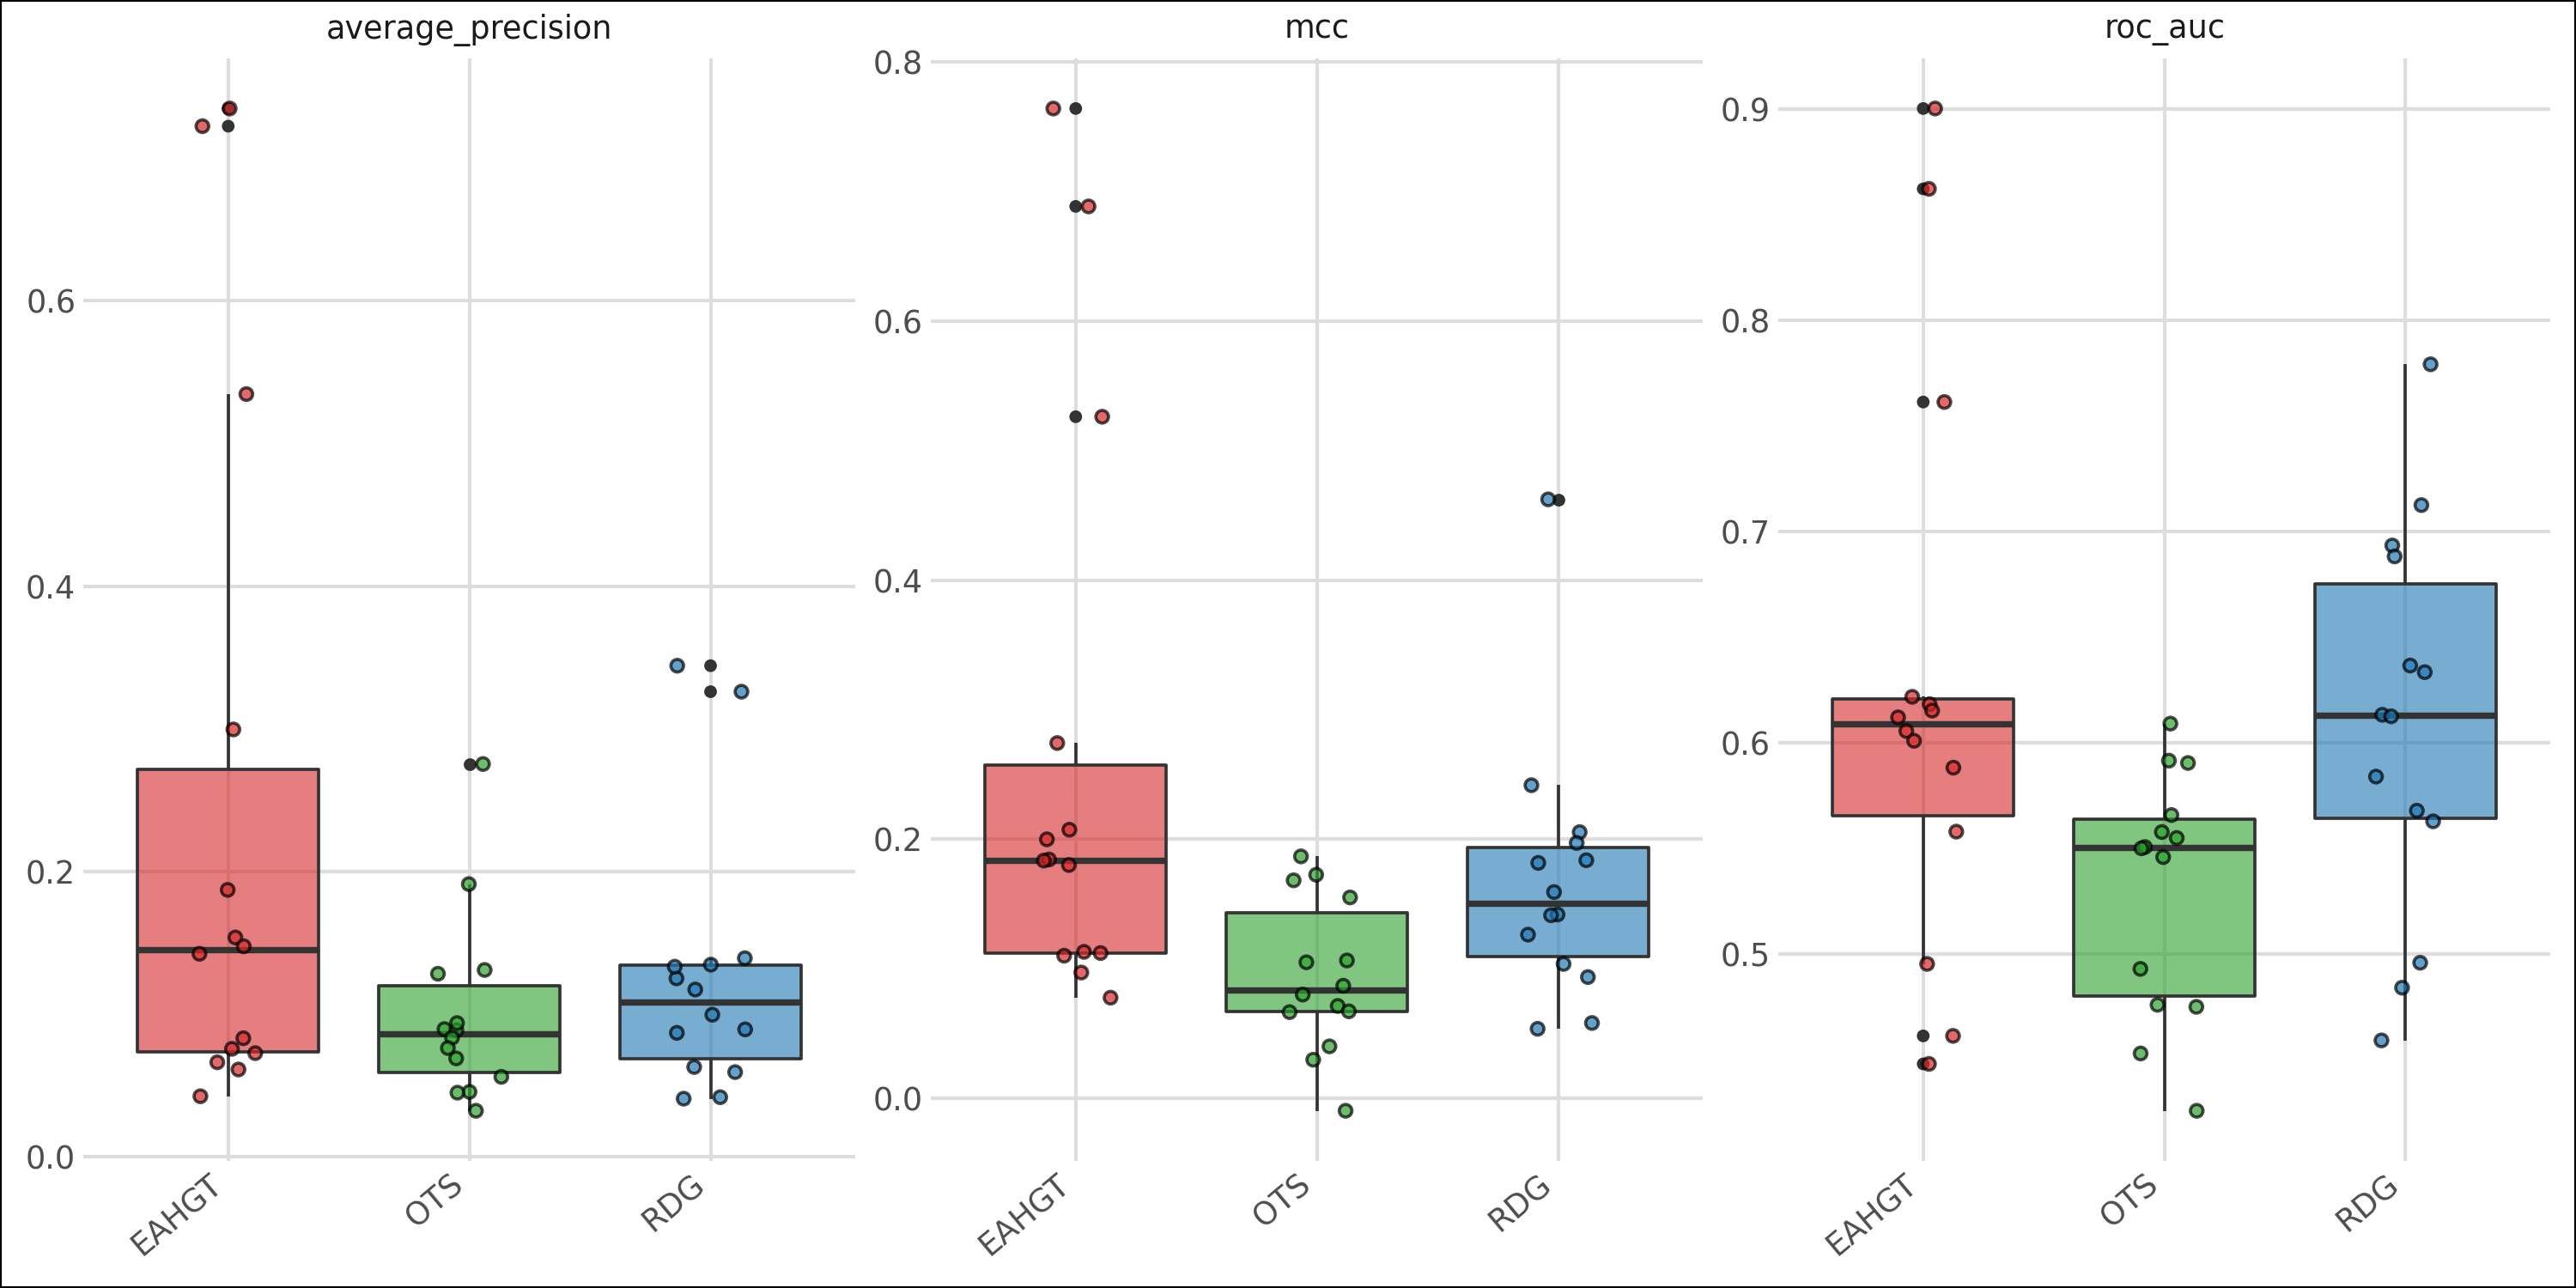
\includegraphics[width=\columnwidth]{figures/results/classification_metrics_by_ta.png}
\caption{Classification metrics (AUROC and average precision) by
therapeutic area for \eahgt{} (P3), RDG, and OTS under decision-aligned
evaluation. Each box summarises the distribution across therapeutic areas;
individual points represent per-area values.}
\label{fig:classification_by_ta}
\end{figure}

\subsubsection{Performance by evidence stratum.}

\begin{figure*}[t]
\centering
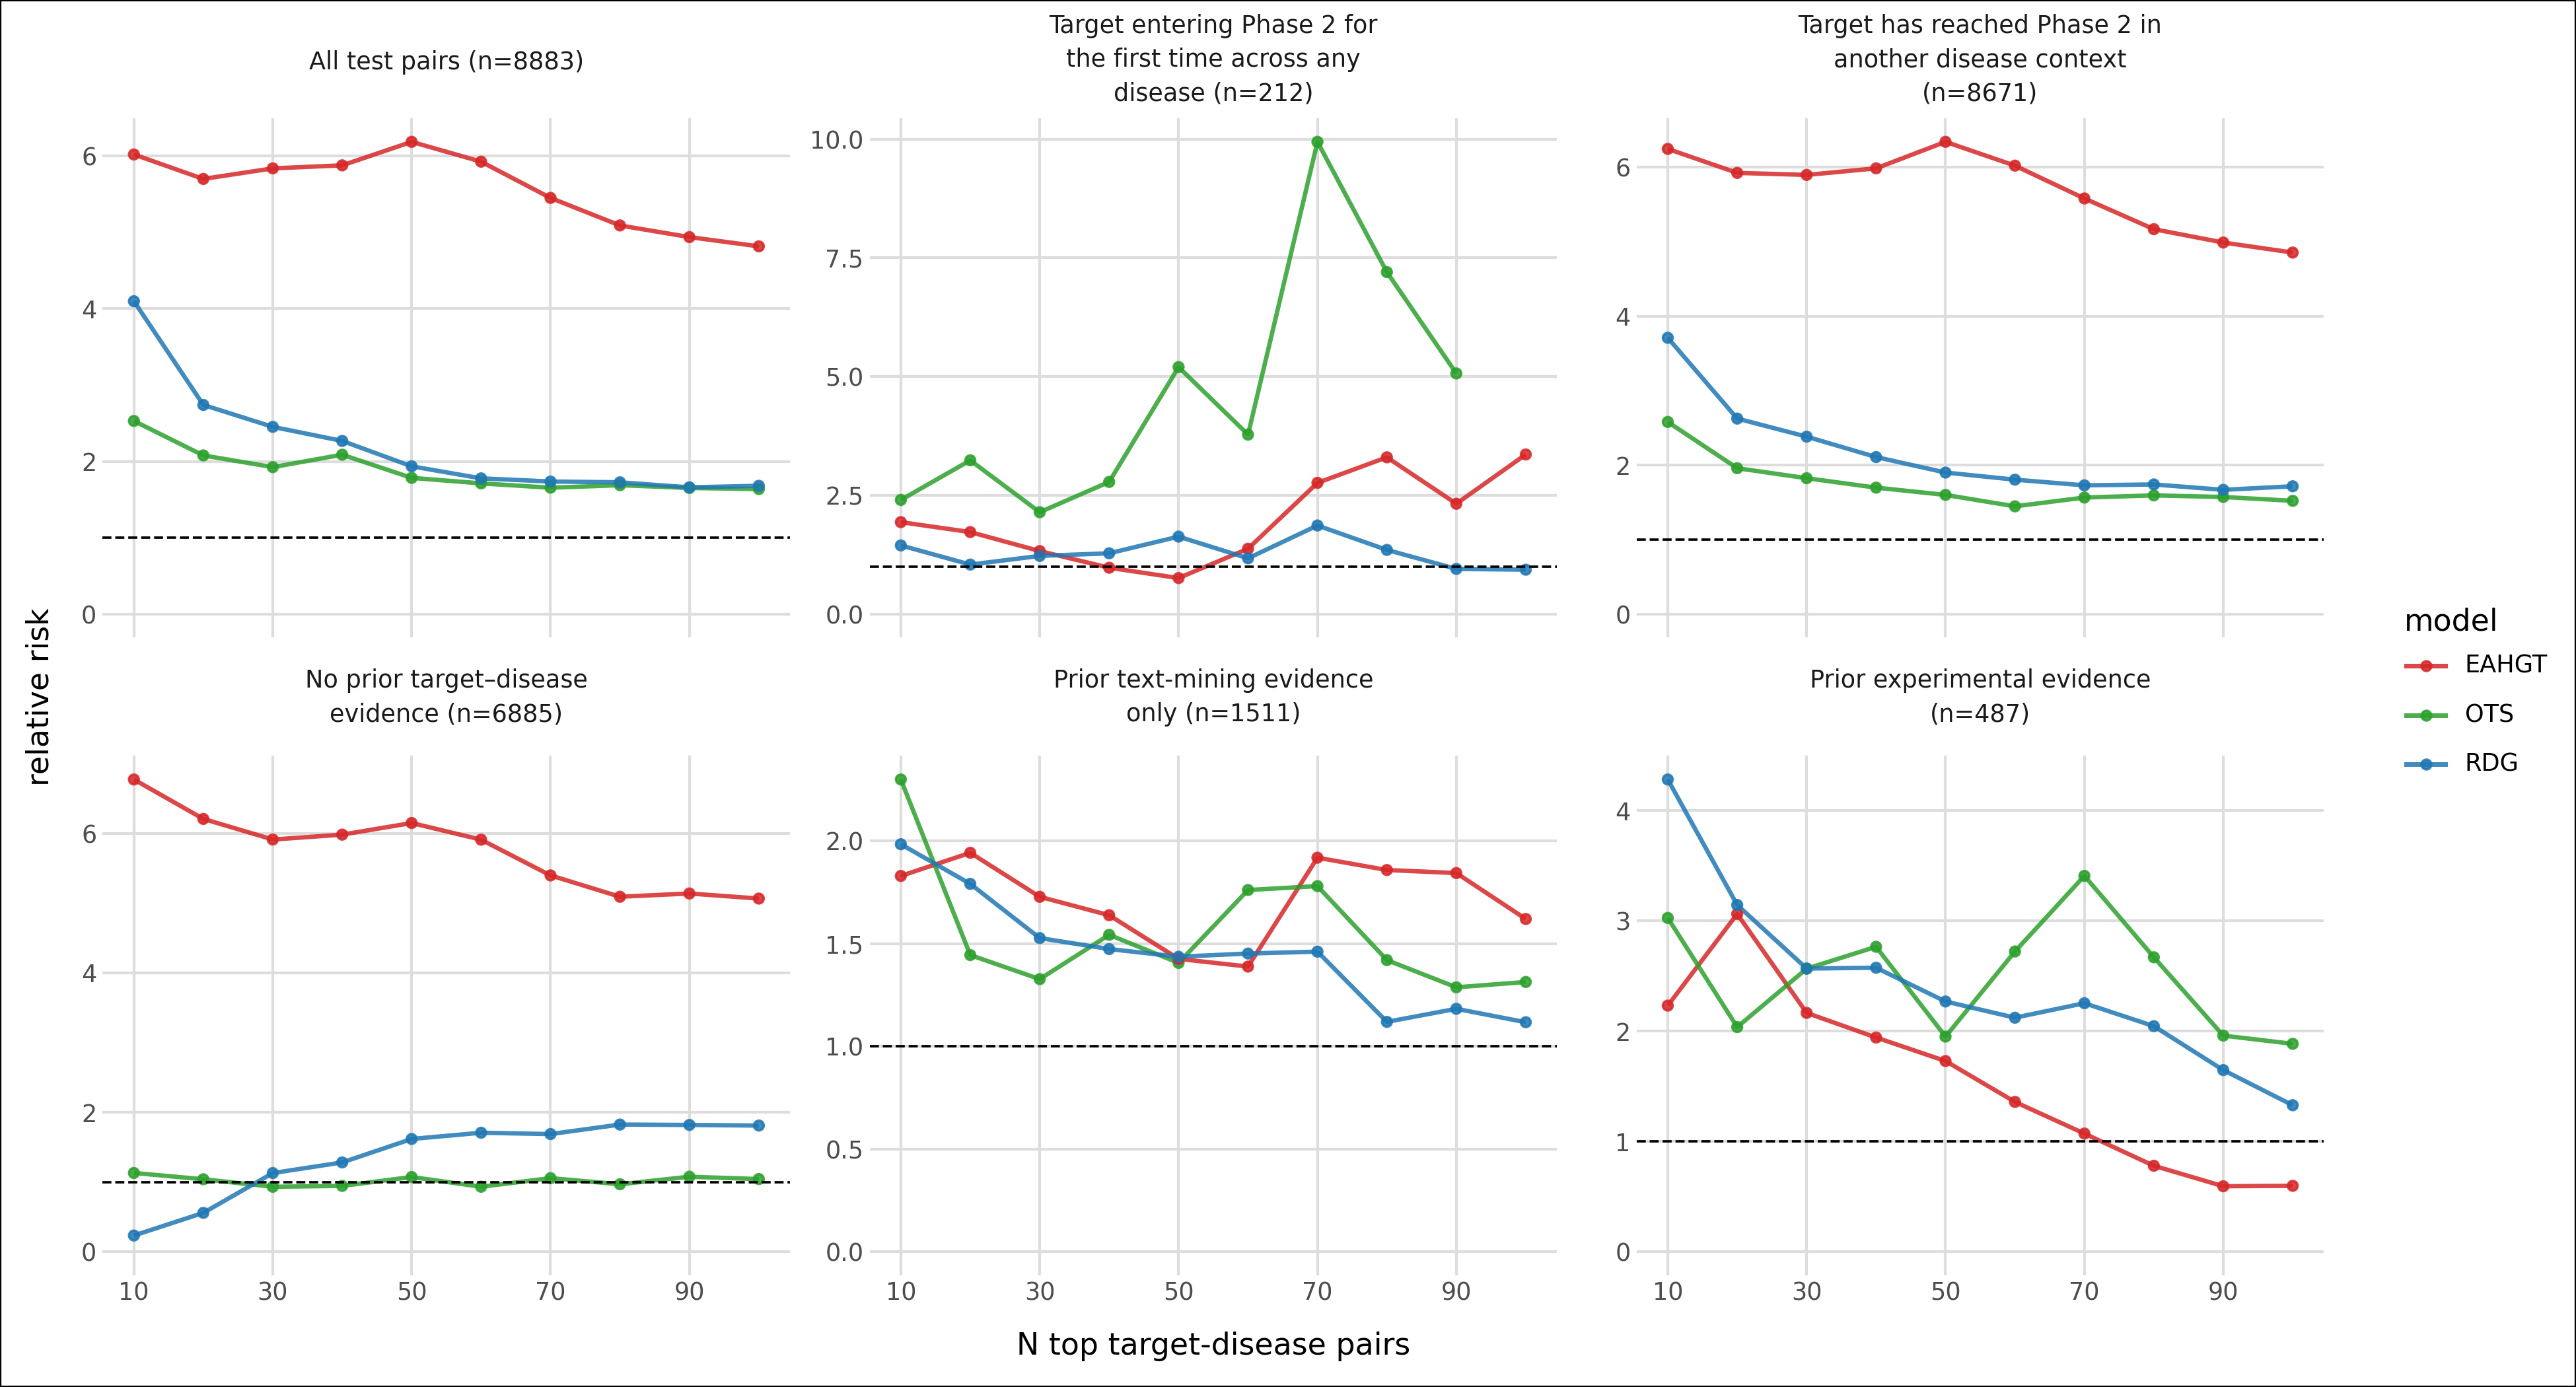
\includegraphics[width=\textwidth]{figures/results/relative_risk_by_limit_by_stratum.png}
\caption{Relative risk by top-$N$ cutoff stratified by evidence
availability at the clinical decision point, for \eahgt{} (P3), RDG,
and OTS. Strata: \textit{evidence\_free} (no direct target--disease
evidence), \textit{literature\_only} (text-mined co-occurrence only),
\textit{direct\_evidence} (experimental evidence present),
\textit{pioneer} (target entering Phase~II for the first time), and
\textit{known} (target has reached Phase~II in another disease context).
Stratum $\times$ TA breakdowns of the classification metrics are
reported in Supplementary Figure~\ref{fig:classification_by_stratum_ta}.}
\label{fig:rr_by_stratum}
\end{figure*}

The advantage of \eahgt{} over RDG is not uniform across strata but is
concentrated precisely where direct-edge models lack signal
(Figure~\ref{fig:rr_by_stratum}). Among pairs with no prior
target--disease evidence of any type at the decision point
(\textit{evidence\_free}), \eahgt{} achieves RR@10 $\approx$ 2.6 while
RDG is near 0.2, essentially no signal. The heterogeneous graph
structure, which encodes multi-hop biological relationships, provides
ranking signal in the complete absence of the direct target--disease links
that RDG relies on. Among pairs supported only by literature
co-occurrence (\textit{literature\_only}), \eahgt{} is 2--3$\times$ RDG
across the full $N$ range: text-mining evidence exists but is weak, and
graph topology augments it substantially. For \textit{pioneer} targets
(first Phase~II entry across any disease), \eahgt{} shows bursts of high
enrichment at specific cutoffs but the curves are noisy (the small
number of pioneer test pairs limits statistical reliability per stratum.

Conversely, for pairs with prior experimental evidence
(\textit{direct\_evidence}), the gap narrows sharply. Both models rank
well at small $N$, but the direct evidence features are dominant, leaving
little room for graph-derived signal to add value. For \textit{known}
targets (prior Phase~II in another disease context), both models perform
well and the curves track more closely, with \eahgt{} maintaining a
modest consistent advantage.

A stratified view of classification metrics by both evidence stratum and
therapeutic area (Supplementary Figure~\ref{fig:classification_by_stratum_ta})
confirms that the \eahgt{} advantage on average precision is most pronounced
in the \textit{evidence\_free} and \textit{literature\_only} strata,
particularly for pioneer targets, cases where RDG has minimal signal and
the graph must fill the gap. The \textit{known} $\times$
\textit{direct\_evidence} intersection is the easiest subpopulation for all
models; \textit{pioneer} $\times$ \textit{evidence\_free} is the hardest.

\subsubsection{Per-therapeutic-area analysis.}

The enrichment advantage of \eahgt{} over RDG is broadly distributed
across therapeutic areas rather than driven by a single area
(Figure~\ref{fig:classification_by_ta}; Supplementary
Figure~\ref{fig:rr_distributions_ta}). At
$N = 10$, \eahgt{} exceeds RDG in nearly every therapeutic area, with
several areas showing RR $>$ 6 (hematologic, immune system, endocrine),
likely driven by dense multi-hop evidence networks in these disease
domains. At $N = 100$, the advantage narrows but remains positive in most
areas, with RDG achieving competitive performance at wider cutoffs where
its linear features remain informative even when graph signal adds less
marginal value. OTS shows moderate enrichment in oncology and
cardiovascular areas but falls behind in disease areas with sparser direct
evidence, consistent with its association-score design.

A Wilcoxon signed-rank test of per-therapeutic-area RR (paired \eahgt{}
vs.\ RDG, one-sided, $n = 13$ TAs) yields $p = 0.16$ at $N = 10$,
$p = 0.05$ at $N = 20$, $p = 0.03$ at $N = 50$, and $p = 0.10$ at
$N = 100$. The \eahgt{} distribution is clearly shifted upward in
every panel --- the per-TA median \eahgt{} RR exceeds the median RDG
RR at all cutoffs (5.60 vs.\ 3.19 at $N = 10$; 2.68 vs.\ 1.77 at
$N = 50$) --- but the right-skewed per-TA distribution has high
variance: a handful of small therapeutic areas in which no
top-ranked \eahgt{} pair advanced (e.g.\ integumentary system
disease, reproductive system or breast disease) hold the paired test
below significance at the tightest and widest cutoffs. The
TA-averaged RR (Table~\ref{tab:rr_main}, the mean rather than the
median over TAs) is pulled up by the high-RR oncology and
hematologic areas and shows a $\geq 2.9\times$ \eahgt{} advantage at
every cutoff. The direction of effect never reverses
(Supplementary Figure~\ref{fig:rr_distributions_ta}).


% Ablation analysis across conditions B1--P3 is in preparation and will
% be added as a subsection here when complete.


% ============================================================
\section{DISCUSSION}
% ============================================================

\subsection{Graph Propagation Recovers Advancement Signal in the Evidence-Sparse Regime}
\label{sec:discussion_sparse_recovery}

The main finding is that \eahgt{}'s advantage over the direct-edge RDG
baseline is concentrated in the strata where feature-based models have
no signal. Among \textit{evidence\_free} pairs (75.4\% of Phase~II
target--disease pairs), RDG achieves RR@10 $\approx$ 0.22, meaning its
ranking is effectively anti-correlated with advancement. \eahgt{}
achieves RR@10 $\approx$ 2.64 on the same pairs. The reason is simple:
RDG receives a zero-valued feature vector for these pairs and cannot
distinguish one from another. The graph encoder, by contrast, aggregates
information from the multi-hop neighbourhood, including shared pathway
memberships, protein interaction partners, and co-targeted molecules with
independent disease associations, producing embeddings that differ between
pairs even when direct evidence is absent.

This validates the coverage expansion that \citet{Falaguera2025TemporalDiscovery}
argued for. They showed that indirect evidence paths increase the
proportion of scoreable targets (44\% with indirect genetic support
vs.\ 23\% direct; 52\% with indirect non-clinical support vs.\ 13\%
direct) but did not build the infrastructure to exploit this for
advancement prediction. The THBKG realises their analysis: the indirect
paths they characterised are the paths through which the graph encoder
recovers signal. Importantly, the recovered signal is not just non-zero
scores for previously unscored pairs. It is \emph{advancement-predictive},
discriminating between pairs that will and will not advance.

The second-largest stratum-level advantage appears in the
\textit{literature\_only} regime, where \eahgt{} delivers 2--3$\times$
the enrichment of RDG. Literature co-occurrence reflects accumulated
research attention rather than mechanistic validity. It dominates among
pairs with any direct evidence (12.5--22.8\% depending on the therapeutic
area) but provides weak discrimination for advancement. The graph encoder
supplements this weak signal with structural context from the broader
neighbourhood, allowing finer-grained ranking among pairs whose literature
scores are similar.

For \textit{direct\_evidence} pairs, the advantage of \eahgt{} diminishes.
RDG achieves competitive enrichment at small $N$ and outperforms \eahgt{}
at mid-range cutoffs. This is expected: when genetic associations, animal
model data, or pathway perturbation results are available, they provide a
strong direct signal of mechanistic relevance, and the graph neighbourhood
adds less. Overall, \eahgt{} outperforms direct-edge models across all
strata, but the margin is largest where direct evidence is absent and
smallest where strong experimental evidence already exists.

The therapeutic area analysis is consistent with this pattern. The largest
per-area gains ($\Delta$RR at $N = 10$: hematologic +15.3, immune system
+10.4, endocrine +8.6) occur in areas with complex multi-target biology
where indirect paths through shared pathways and protein interaction
networks carry useful information. Areas with marginal or reversed
advantages at deep cutoffs (respiratory, urinary) tend to have smaller
evaluation sets and sparser graph neighbourhoods, suggesting that the
benefit of multi-hop propagation depends on the structural richness of
the local graph.


\subsection{Continuation Work}
\label{sec:discussion_continuation}

Several directions for extending the present work are under active
investigation.

\textbf{Quantifying temporal inflation risk.} The decision-aligned
evaluation protocol of \citet{Czech2024CLINICALFORECASTING} removes temporal leakage, but
the magnitude of the inflation it prevents has not been directly
quantified. A natural experiment would be to compare calendar-split
evaluation (a single global cutoff for all pairs) against per-instance
masking on the same model and test set. However, this comparison is
confounded: under calendar split, pairs that entered Phase~II well before
the global cutoff absorb more post-decision evidence into their features,
but they also have more complete advancement labels. Feature inflation
and label completeness cannot be separated.

We therefore plan a shifted-offset experiment that isolates the effect
of evidence inflation while holding labels fixed. For each pair with
Phase~II entry year $y$, we reconstruct the evidence subgraph at shifted
cutoffs $y + \delta$ for $\delta \in \{-5, -3, -1, 0, +1, +3, +5, +10\}$
and re-evaluate. Positive offsets simulate post-decision evidence leakage:
if successful targets attract accelerated publication and curation, their
subgraphs will grow faster than those of unsuccessful targets at
$\delta > 0$, inflating discriminative performance. Negative offsets
characterise how quickly signal degrades as the evidence window is
truncated before the decision point. The gap between $\delta = 0$ and
large positive $\delta$ quantifies inflation risk; the gap between
$\delta = 0$ and negative $\delta$ characterises signal arrival timing.
Jointly, the positive and negative offset curves define an inflation
envelope within which the true quasi-prospective performance of any
evidence-based model must lie. Comparing this envelope for \eahgt{}
versus RDG will reveal whether graph-based models are more or less
susceptible to inflation than direct-edge models. This analysis requires
only the existing THBKG temporal masking infrastructure applied at shifted
cutoffs, with no additional data collection.

\textbf{Open Targets 25.06 update.} All data, graph construction, and
baseline comparison scores are currently anchored at Open Targets release
23.06. The full pipeline (edge collection, graph construction, node
feature engineering, model training, and evaluation) will be re-run
against the latest 25.06 release to ensure that results reflect current
evidence coverage and curation state. This update is particularly
important for clinical trial edges, which are among the most rapidly
growing evidence categories \citep{Falaguera2025TemporalDiscovery}, and for genetic
association evidence, where the ongoing expansion of UK Biobank and
FinnGen credible sets substantially increases coverage for previously
under-annotated therapeutic areas.

\textbf{Ablation analysis.} The results presented here compare the best
\eahgt{} configuration (P3: both cumulative score and novelty score
features, LambdaRank loss) against the external RDG baseline. A systematic ablation
across all eight conditions defined in Table~\ref{tab:conditions}
(B1--B5, P1--P3) is in preparation and will isolate the contributions of
three independent architectural choices: (i) heterogeneous attention
(\hgt{} vs.\ \gatv{} via \texttt{HeteroConv}), (ii) temporal encoding
(RTE vs.\ explicit novelty score vs.\ both), and (iii) edge feature
integration (multiplicative modulation vs.\ concatenation vs.\ none). Of particular
interest is the comparison between B2 (\hgtrte{}) and P2/P3, which will
reveal whether the learned temporal encoding of RTE and the explicit
novelty scalar $n_{ij}$ capture overlapping or complementary temporal
dynamics.

\textbf{Practical application: clinical portfolio optimisation.} The
primary application of advancement prediction is scoring existing Phase~II
programmes against the current evidence landscape to support resource
allocation decisions. A key value of the graph-based approach is its
ability to characterise programmes whose direct evidence record is thin at
the decision point, the 75.4\% of pairs that direct-edge models cannot
score. For these under-evidenced programmes, the THBKG provides a
differentiated assessment based on indirect structural support: pathway
context, protein interaction partners, functional annotations, and drug
modulation profiles. This allows decision-makers to distinguish between
programmes that are under-evidenced because the curation record lags
behind the biology, and programmes that lack structural support in the
graph neighbourhood. Target prioritisation models such as GATher
\citep{Narganes-Carlon2024GATher:Links} and PWAS
\citep{Narganes-Carlon2023ATargets} predict max clinical phase across the full
gene--disease space, addressing the broader question of which targets to
pursue; advancement prediction addresses the narrower but complementary
question of which existing programmes are best supported for progression.
Whether the advancement signal learned under temporal constraints
transfers to forward-looking scoring of undeveloped target--disease pairs is
an open question that planned follow-up work will address.


% ============================================================
\section{CONCLUSION}
% ============================================================

%TODO


% ============================================================
\section{ACKNOWLEDGEMENTS}
% ============================================================

%TODO

\subsubsection{Conflict of interest statement.} None declared.

\newpage

\bibliographystyle{unsrtnat}  % TODO: replace with 'nar' once nar.bst is added to project
\bibliography{reference}


% ============================================================
\clearpage
\onecolumn
\section*{SUPPLEMENTARY MATERIAL}
% ============================================================

\begin{table}[h]
\caption{Full edge type specification for the THBKG. All temporal edges
carry a two-dimensional attribute $[s_{ij}, n_{ij}]$ (cumulative score
and Open Targets novelty score) and a snapshot year. Static edges carry
$[0.0, 1.0]$ and no timestamp. Clinical trial and advancement edges are
excluded from the GNN context graph to prevent label leakage.}
\label{tab:edge_types_full}
\centering
\begin{tabular}{llllrl}
\toprule
\textbf{Category} & \textbf{Relation} & \textbf{Src} & \textbf{Dst} &
\textbf{Count} & \textbf{Data sources} \\
\midrule
\multirow{6}{*}{\rotatebox[origin=c]{90}{\parbox{2.2cm}{\centering Target--disease\\evidence}}}
& \texttt{genetic\_association}  & target & disease & 82{,}408  & GWAS, EVA, ClinGen, gene burden, Genomics England, gene2phenotype, UniProt, Orphanet \\
& \texttt{animal\_model}         & target & disease & 442{,}082 & IMPC \\
& \texttt{literature}            & target & disease & 237{,}795 & EuropePMC \\
& \texttt{rna\_expression}       & target & disease & 171{,}555 & Expression Atlas \\
& \texttt{somatic\_mutation}     & target & disease & 63{,}557  & Cancer Gene Census, IntOGen, EVA somatic \\
& \texttt{affected\_pathway}     & target & disease & 38{,}804  & Reactome, CRISPR screen, SLAPenrich, PROGENy \\
\midrule
\multirow{4}{*}{\rotatebox[origin=c]{90}{\parbox{2.0cm}{\centering Clinical\\trials}}}
& \texttt{ct\_positive}          & disease & target & 56{,}190 & ChEMBL; \texttt{clinicalStatus} = completed \\
& \texttt{ct\_unknown}           & disease & target & 52{,}738 & ChEMBL; administrative or operational \\
& \texttt{ct\_unmet\_efficacy}   & disease & target &  4{,}240 & ChEMBL; stop reason contains `negative' \\
& \texttt{ct\_adverse\_effects}  & disease & target &  2{,}115 & ChEMBL; stop reason contains `safety' \\
\midrule
\multirow{5}{*}{\rotatebox[origin=c]{90}{\parbox{2.5cm}{\centering Pathway,\\functional,\\molecular}}}
& \texttt{interacts\_with}       & target & target   & 659{,}444 & IntAct (protein--protein interaction) \\
& \texttt{has\_function\_in}     & target & go       & 256{,}090 & Gene Ontology annotations \\
& \texttt{modulated\_by}         & target & molecule &  45{,}416 & ChEMBL compound--target activity \\
& \texttt{involved\_in}          & target & reactome &  36{,}972 & Reactome, SLAPenrich \\
& \texttt{associated\_with}      & disease & reactome &  3{,}639 & Reactome, SLAPenrich \\
\midrule
Label
& \texttt{advancement}           & target & disease &  34{,}410 & ChEMBL (derived); excluded from context graph \\
\midrule
\multirow{3}{*}{\rotatebox[origin=c]{90}{\parbox{1.5cm}{\centering Static\\ontology}}}
& \texttt{is\_subtype\_of}       & disease & disease     & 11{,}548 & EFO / Disease Ontology \\
& \texttt{is\_subtype\_of}       & go & go               & 14{,}415 & Gene Ontology (\texttt{is\_a}) \\
& \texttt{is\_subpathway\_of}    & reactome & reactome   &    492   & Reactome \\
\bottomrule
\end{tabular}
\end{table}

\begin{figure}[h]
\centering
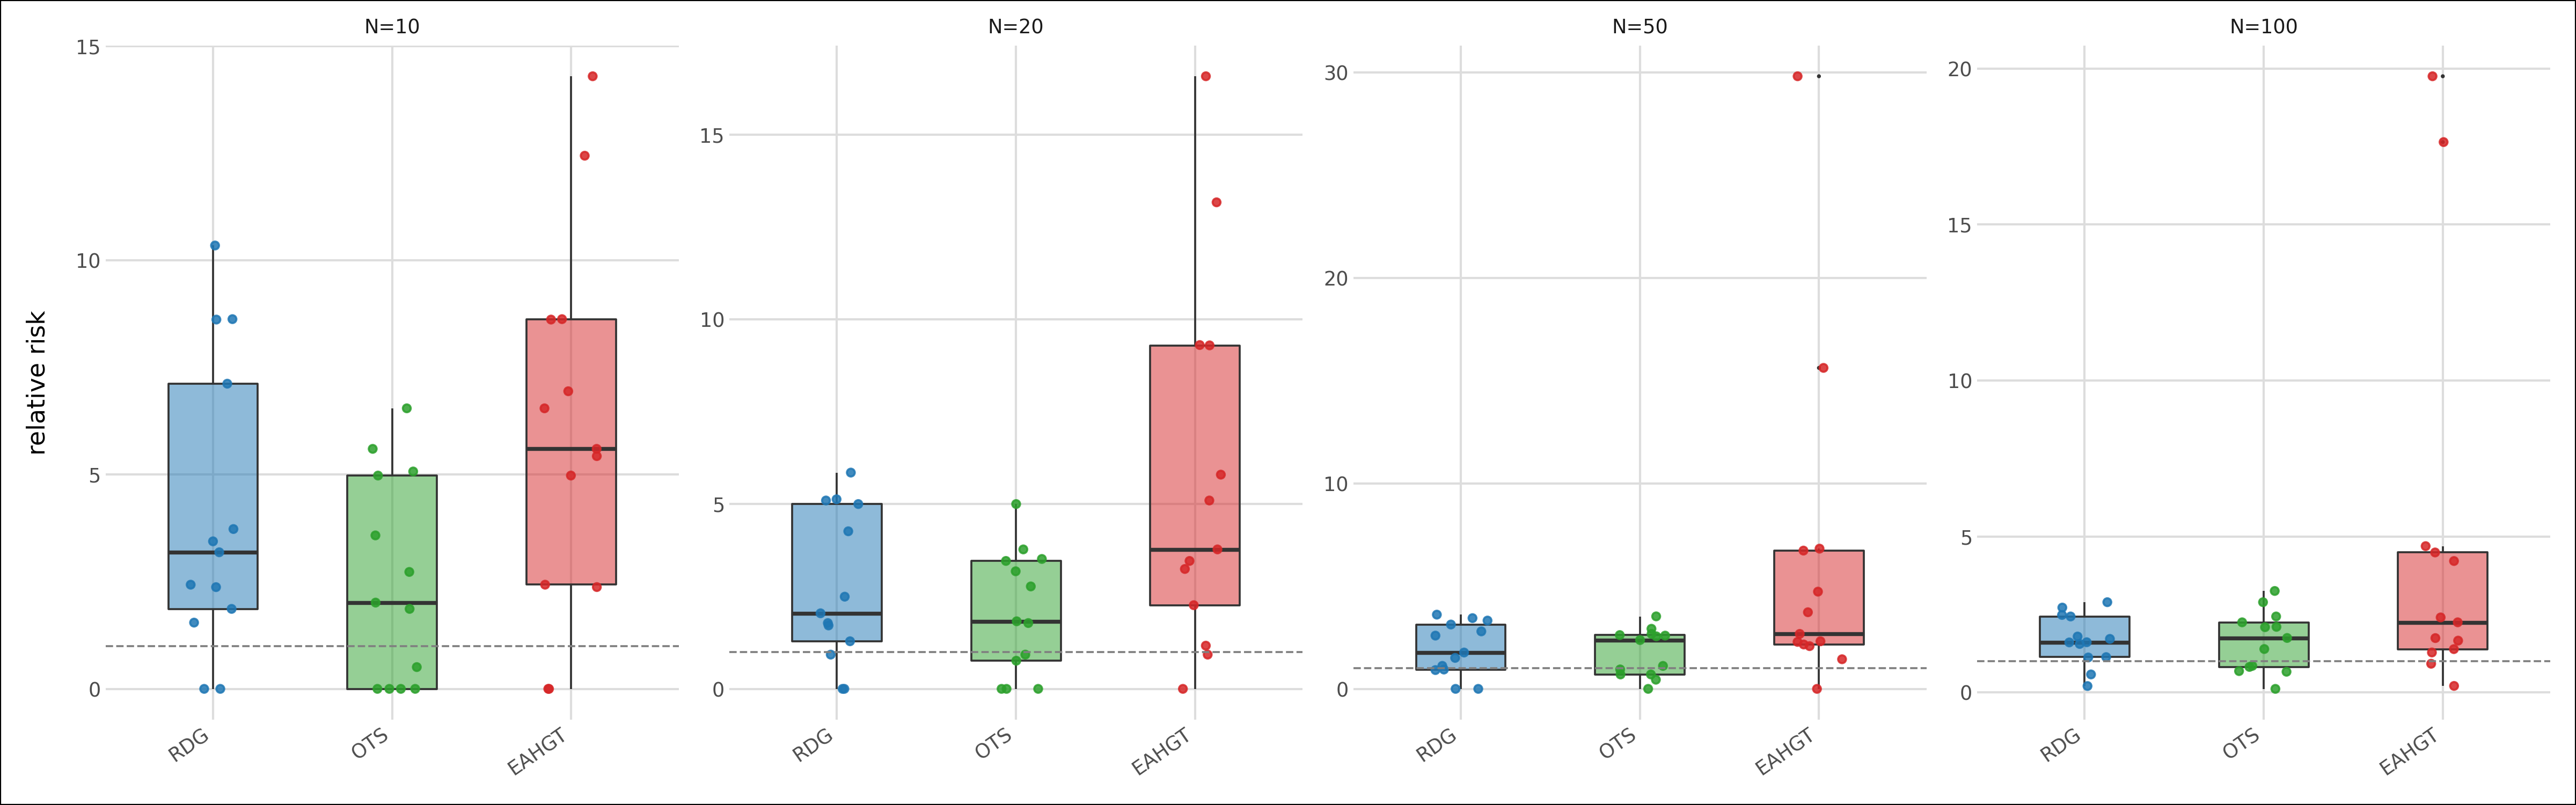
\includegraphics[width=0.8\textwidth]{figures/results/rr_distributions_ta.png}
\caption{Box-plot distributions of RR@$N$ across therapeutic areas for
\eahgt{} (P3), RDG, and OTS at $N \in \{10, 20, 50, 100\}$. Each dot is
one primary therapeutic area; the box shows median and IQR. The dashed
line marks RR $=1$ (no enrichment). \eahgt{} has the highest median RR
in every panel.}
\label{fig:rr_distributions_ta}
\end{figure}

\begin{figure}[h]
\centering
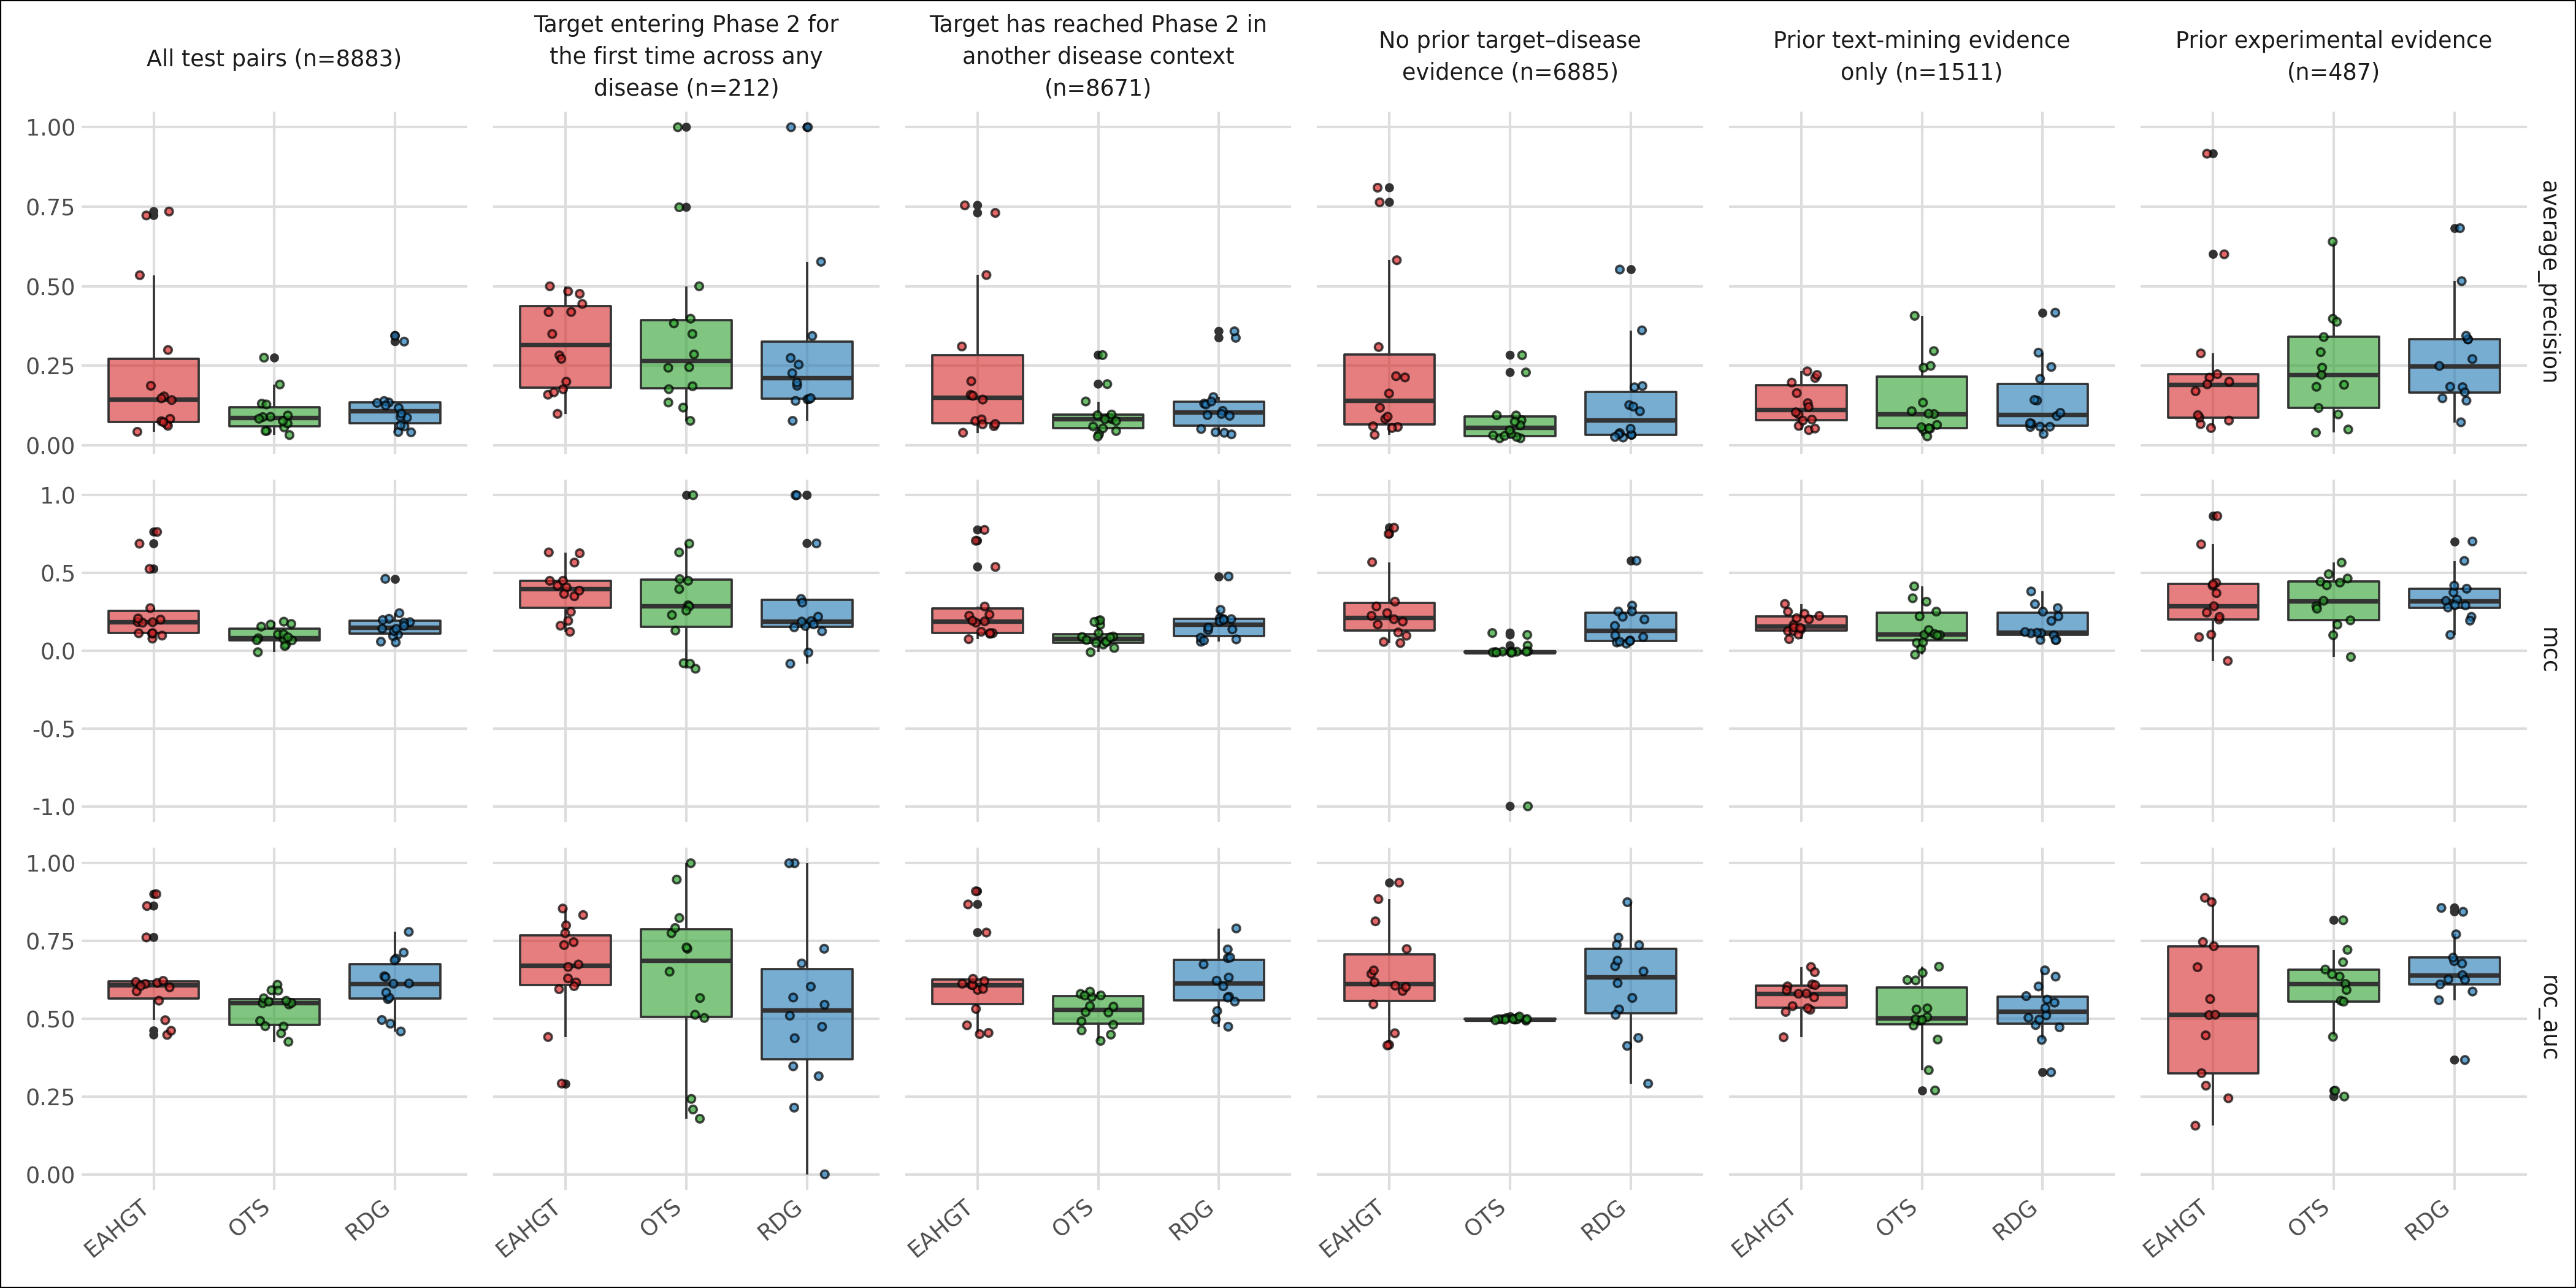
\includegraphics[width=0.8\textwidth]{figures/results/classification_metrics_by_stratum_by_ta.png}
\caption{Classification metrics (AUROC and average precision) stratified
by both evidence stratum (pioneer/known, evidence density) and therapeutic
area. The \eahgt{} advantage on AP is most pronounced in the
\textit{evidence\_free} and \textit{literature\_only} strata for pioneer
targets.}
\label{fig:classification_by_stratum_ta}
\end{figure}

\end{document}